\appendix


\chapter{\emph{Source code} program}

\section{main\_integer.py }

\begin{lstlisting}[language=Python, basicstyle=\tiny]
	import numpy as np
	import matplotlib.pyplot as plt
	from skimage.color import rgb2gray
	from skimage.filters import gaussian, sobel
	from skimage.io import imread
	
	my_dpi = 96 # https://www.infobyip.com/detectmonitordpi.php
	
	# input data
	kategori = "luka_merah"
	path = "dataset_3/"+kategori+"/ready/"
	path_skripsi = "D:/RL/skripsweet/dataset/dataset_3/"+ kategori +"/ready/"
	img_name = "42"
	extension = ".jpg"
	img = imread(path + img_name + extension)
	im_gray = rgb2gray(img)
	im_gt = imread(path + img_name + "_g" + extension)
	
	
	# parameter set
	cr=160
	cc=180
	rad=90
	sigma=3.5
	sample=100
	alpha = 1
	beta = 10
	gamma = 2 # time step
	max_iter=100
	
	# snake init (circle)
	theta = np.linspace(0, 2*np.pi, sample)
	r = cr + rad*np.sin(theta)
	c = cc + rad*np.cos(theta)
	snake_init = np.array([r, c]).T
	snake_init = np.around(snake_init).astype(int)
	
	snake_xy = snake_init[:, ::-1].astype(int)
	x = snake_xy[:, 0].astype(int)
	y = snake_xy[:, 1].astype(int)
	n = len(x)
	
	fig0= plt.figure(frameon=False, figsize=(img.shape[1]/my_dpi, img.shape[0]/my_dpi), dpi=my_dpi)
	ax0 = fig0.add_axes([0, 0, 1, 1])
	ax0.imshow(im_gray, cmap=plt.cm.gray)
	ax0.plot(snake_xy[:, 0], snake_xy[:, 1], '-r', lw=2)
	ax0.set_xticks([]), ax0.set_yticks([]) # hide axes
	ax0.axis('off')
	outname0 = path + img_name +"_integer_init"+ extension
	outname0_skripsi = path_skripsi + img_name +"_integer_init"+ extension
	plt.savefig(outname0, dpi=my_dpi)
	plt.savefig(outname0_skripsi, dpi=my_dpi)
	print(outname0 + " has been saved")
	print(outname0_skripsi + " has been saved")
	plt.close(fig0)
	
	
	# energy external
	ext = gaussian(im_gray, sigma)
	ext = sobel(ext)
	ext = -ext**2
	
	# save energy external
	fig1= plt.figure(frameon=False, figsize=(img.shape[1]/my_dpi, img.shape[0]/my_dpi), dpi=my_dpi)
	ax1 = fig1.add_axes([0, 0, 1, 1])
	ax1.imshow(ext, cmap=plt.cm.gray)
	ax1.set_xticks([]), ax1.set_yticks([]) # hide axes
	ax1.axis('off')
	outname1 = path + img_name +"_integer_ext"+ extension
	outname1_skripsi = path_skripsi + img_name +"_integer_ext"+ extension
	plt.savefig(outname1, dpi=my_dpi)
	plt.savefig(outname1_skripsi, dpi=my_dpi)
	print(outname1 + " has been saved")
	print(outname1_skripsi + " has been saved")
	plt.close(fig1)
	
	
	# energy internal
	# matrix
	a = beta
	b = -(4*beta + alpha)
	c = 6*beta + 2*alpha
	
	eye_n = np.eye(n, dtype=float)
	
	c_axis = c * eye_n
	b_axis = b * ( np.roll(eye_n, -1, axis=0) + np.roll(eye_n, -1, axis=1) )
	a_axis = a * ( np.roll(eye_n, -2, axis=0) + np.roll(eye_n, -2, axis=1) )
	
	A = c_axis + b_axis + a_axis
	inv = np.linalg.inv(eye_n + gamma * A) # acton, ivins matrix equation
	
	# potential force
	gy, gx = np.gradient(ext)
	
	# deform snake
	fig2= plt.figure(frameon=False, figsize=(img.shape[1]/my_dpi, img.shape[0]/my_dpi), dpi=my_dpi)
	ax2 = fig2.add_axes([0, 0, 1, 1])
	ax2.imshow(im_gray, cmap=plt.cm.gray)
	
	xt = np.copy(x)
	yt = np.copy(y)
	
	for i in range(max_iter):
	fx = np.array([])
	fy = np.array([])
	
	for i in range(n):
	fx = np.append(fx, gx[yt[i]] [xt[i]] )
	fy = np.append(fy, gy[yt[i]] [xt[i]] )
	
	xn = np.dot(inv, xt + gamma * fx) # acton, ivins equation
	yn = np.dot(inv, yt + gamma * fy)
	
	xt = np.round(xn).astype(int)
	yt = np.round(yn).astype(int)
	
	# ax2.plot(xt, yt, '-g', lw=2)
	
	snake_final = np.array([xt, yt]).T
	
	ax2.plot(snake_xy[:, 0], snake_xy[:, 1], '-r', lw=2)
	ax2.plot(snake_final[:, 0], snake_final[:, 1], '-b', lw=2)
	ax2.set_xticks([]), ax2.set_yticks([]) # hide axes
	ax2.axis('off')
	outname2 = path + img_name +"_integer_result"+ extension
	outname2_skripsi = path_skripsi + img_name +"_integer_result"+ extension
	plt.savefig(outname2, dpi=my_dpi)
	plt.savefig(outname2_skripsi, dpi=my_dpi)
	print(outname2 + " has been saved")
	print(outname2_skripsi + " has been saved")
	# plt.show()
	plt.close(fig2)
	
	# save final contour region
	fig3= plt.figure(frameon=False, figsize=(img.shape[1]/my_dpi, img.shape[0]/my_dpi), dpi=my_dpi)
	ax3 = fig3.add_axes([0, 0, 1, 1])
	ax3.imshow(np.ones(img.shape))
	ax3.fill(snake_final[:, 0], snake_final[:, 1], color="black")
	ax3.set_xticks([]), ax3.set_yticks([]) # hide axes
	ax3.axis('off')
	outname3 = path + img_name +"_integer_r"+ extension
	outname3_skripsi = path_skripsi + img_name +"_integer_r"+ extension
	plt.savefig(outname3, dpi=my_dpi)
	plt.savefig(outname3_skripsi, dpi=my_dpi)
	print(outname3 + " has been saved")
	print(outname3_skripsi + " has been saved")
	plt.close(fig3)
	
	
	# save overlay groundtruth & final snake
	
	fig4= plt.figure(frameon=False, figsize=(img.shape[1]/my_dpi, img.shape[0]/my_dpi), dpi=my_dpi)
	ax4 = fig4.add_axes([0, 0, 1, 1])
	ax4.imshow(im_gt, cmap=plt.cm.gray)
	ax4.plot(snake_final[:, 0], snake_final[:, 1], '-b', lw=2)
	ax4.set_xticks([]), ax4.set_yticks([]) # hide axes
	ax4.axis('off')
	outname4 = path + img_name +"_gt_r_integer"+ extension
	outname4_skripsi = path_skripsi + img_name +"_gt_r_integer"+ extension
	plt.savefig(outname4, dpi=my_dpi)
	plt.savefig(outname4_skripsi, dpi=my_dpi)
	print(outname4 + " has been saved")
	print(outname4_skripsi + " has been saved")
	plt.close(fig4)
\end{lstlisting}


\section{main\_interpolation.py}
\begin{lstlisting}[language=Python, basicstyle=\tiny]
	import numpy as np
	import matplotlib.pyplot as plt
	from skimage.color import rgb2gray
	from skimage.util import img_as_float
	from skimage.filters import gaussian, sobel
	from skimage.io import imread
	from scipy.interpolate import RectBivariateSpline
	# skimage version 0.19.3
	
	my_dpi = 96 # https://www.infobyip.com/detectmonitordpi.php
	
	# input data
	path = "dataset_3/luka_hitam/ready/"
	path_skripsi = "D:/RL/skripsweet/dataset/dataset_3/luka_hitam/ready/"
	img_name = "37"
	extension = ".jpg"
	img = imread(path + img_name + extension)
	im_gray = rgb2gray(img)
	im_gt = imread(path + img_name + "_g" + extension)
	
	# parameter set
	cr=110
	cc=125
	rad=80
	sigma=3.5
	sample=400
	alpha = 0.015
	beta = 10
	gamma = 0.001 # time step
	max_num_iter=500
	
	
	# snake init (circle)
	theta = np.linspace(0, 2*np.pi, sample)
	r = cr + rad*np.sin(theta)
	c = cc + rad*np.cos(theta)
	snake_init = np.array([r, c]).T
	
	snake_xy = snake_init[:, ::-1]
	x = snake_xy[:, 0].astype(float)
	y = snake_xy[:, 1].astype(float)
	n = len(x)
	
	fig0= plt.figure(frameon=False, figsize=(img.shape[1]/my_dpi, img.shape[0]/my_dpi), dpi=my_dpi)
	ax0 = fig0.add_axes([0, 0, 1, 1])
	ax0.imshow(im_gray, cmap=plt.cm.gray)
	ax0.plot(snake_xy[:, 0], snake_xy[:, 1], '-r', lw=2)
	ax0.set_xticks([]), ax0.set_yticks([]) # hide axes
	ax0.axis('off')
	outname0 = path + img_name +"_interp_init"+ extension
	outname0_skripsi = path_skripsi + img_name +"_interp_init"+ extension
	plt.savefig(outname0, dpi=my_dpi)
	plt.savefig(outname0_skripsi, dpi=my_dpi)
	print(outname0 + " has been saved")
	print(outname0_skripsi + " has been saved")
	plt.close(fig0)
	
	
	# energy external
	ext = gaussian(im_gray, sigma)
	ext = img_as_float(ext)
	ext = ext.astype(float, copy=False)
	ext = sobel(ext)
	
	# save energy external
	fig1= plt.figure(frameon=False, figsize=(img.shape[1]/my_dpi, img.shape[0]/my_dpi), dpi=my_dpi)
	ax1 = fig1.add_axes([0, 0, 1, 1])
	ax1.imshow(ext, cmap=plt.cm.gray)
	ax1.set_xticks([]), ax1.set_yticks([]) # hide axes
	ax1.axis('off')
	outname1 = path + img_name +"_interp_ext"+ extension
	outname1_skripsi = path_skripsi + img_name +"_interp_ext"+ extension
	plt.savefig(outname1, dpi=my_dpi)
	plt.savefig(outname1_skripsi, dpi=my_dpi)
	print(outname1 + " has been saved")
	print(outname1_skripsi + " has been saved")
	plt.close(fig1)
	
	
	# energy internal
	
	a = beta
	b = -(4*beta + alpha)
	c = 6*beta + 2*alpha
	
	eye_n = np.eye(n, dtype=float)
	c_axis = c * eye_n
	b_axis = b * ( np.roll(eye_n, -1, axis=0) + np.roll(eye_n, -1, axis=1) )
	a_axis = a * ( np.roll(eye_n, -2, axis=0) + np.roll(eye_n, -2, axis=1) )
	A = c_axis + b_axis + a_axis
	
	# Only one inversion is needed for implicit spline energy minimization. skimage
	inv = np.linalg.inv(A + gamma * eye_n)
	inv = inv.astype(float, copy=False)
	
	
	# potential force
	gy, gx = np.gradient(ext)
	
	# Interpolate for smoothness
	intp1 = RectBivariateSpline(np.arange(gx.shape[1]),
	np.arange(gx.shape[0]),
	gx.T, kx=2, ky=2, s=0)
	
	intp2 = RectBivariateSpline(np.arange(gy.shape[1]),
	np.arange(gy.shape[0]),
	gy.T, kx=2, ky=2, s=0)
	
	
	# deform snake
	max_px_move=1.0
	
	fig2= plt.figure(frameon=False, figsize=(img.shape[1]/my_dpi, img.shape[0]/my_dpi), dpi=my_dpi)
	ax2 = fig2.add_axes([0, 0, 1, 1])
	ax2.imshow(im_gray, cmap=plt.cm.gray)
	
	xt = np.copy(x)
	yt = np.copy(y)
	
	for i in range(max_num_iter):
	# fx & fy
	fx = intp1(xt, yt, dx=0, grid=False).astype(float, copy=False)
	fy = intp2(xt, yt, dy=0, grid=False).astype(float, copy=False)
	
	# skimage equation
	xn = np.dot(inv, gamma * xt + fx)
	yn = np.dot(inv, gamma * yt + fy)
	
	# Movements are capped to max_px_move per iteration. skimage
	dx = max_px_move * np.tanh(xn - xt)
	dy = max_px_move * np.tanh(yn - yt)
	
	xt += dx
	yt += dy
	
	# if i % 10 == 0:
	#         snake_iter = np.array([xt, yt]).T
	#         ax2.plot(snake_iter[:, 0], snake_iter[:, 1], '-g', lw=2)
	
	snake_final = np.array([xt, yt]).T
	
	ax2.plot(snake_xy[:, 0], snake_xy[:, 1], '-r', lw=2)
	ax2.plot(snake_final[:, 0], snake_final[:, 1], '-b', lw=2)
	ax2.set_xticks([]), ax2.set_yticks([]) # hide axes
	ax2.axis('off')
	outname2 = path + img_name +"_interp_result"+ extension
	outname2_skripsi = path_skripsi + img_name +"_interp_result"+ extension
	plt.savefig(outname2, dpi=my_dpi)
	plt.savefig(outname2_skripsi, dpi=my_dpi)
	print(outname2 + " has been saved")
	print(outname2_skripsi + " has been saved")
	# plt.show()
	plt.close(fig2)
	
	# save final contour region
	fig3= plt.figure(frameon=False, figsize=(img.shape[1]/my_dpi, img.shape[0]/my_dpi), dpi=my_dpi)
	ax3 = fig3.add_axes([0, 0, 1, 1])
	ax3.imshow(np.ones(img.shape))
	ax3.fill(snake_final[:, 0], snake_final[:, 1], color="black")
	ax3.set_xticks([]), ax3.set_yticks([]) # hide axes
	ax3.axis('off')
	outname3 = path + img_name +"_interp_r"+ extension
	outname3_skripsi = path_skripsi + img_name +"_interp_r"+ extension
	plt.savefig(outname3, dpi=my_dpi)
	plt.savefig(outname3_skripsi, dpi=my_dpi)
	print(outname3 + " has been saved")
	print(outname3_skripsi + " has been saved")
	plt.close(fig3)
	
	# save overlay ground truth & final snake
	
	fig4= plt.figure(frameon=False, figsize=(img.shape[1]/my_dpi, img.shape[0]/my_dpi), dpi=my_dpi)
	ax4 = fig4.add_axes([0, 0, 1, 1])
	ax4.imshow(im_gt, cmap=plt.cm.gray)
	ax4.plot(snake_final[:, 0], snake_final[:, 1], '-b', lw=2)
	ax4.set_xticks([]), ax4.set_yticks([]) # hide axes
	ax4.axis('off')
	outname4 = path + img_name +"_gt_r"+ extension
	outname4_skripsi = path_skripsi + img_name +"_gt_r"+ extension
	plt.savefig(outname4, dpi=my_dpi)
	plt.savefig(outname4_skripsi, dpi=my_dpi)
	print(outname4 + " has been saved")
	print(outname4_skripsi + " has been saved")
	plt.close(fig4)
\end{lstlisting}

\section{integer\_validation.py}
\begin{lstlisting}[language=Python, basicstyle=\tiny]
	import numpy as np
	from skimage.color import rgb2gray
	from skimage.io import imread
	import matplotlib.pyplot as plt
	
	
	path = "dataset_3/luka_merah/ready/"
	img_name = "36"
	extension = ".jpg"
	
	groundtruth = rgb2gray(imread(path + img_name + "_r" + extension))
	interp_region = rgb2gray(imread(path + img_name + "_integer_r" + extension))
	
	sum_gt = 0
	sum_interp = 0
	
	for x in groundtruth:
	for y in x:
	if y != 1.0:
	sum_gt += 1
	
	for p in interp_region:
	for q in p:
	if q != 1.0:
	sum_interp += 1
	
	print(sum_gt)
	print(abs(sum_gt-sum_interp))
	print(abs(sum_gt-sum_interp) / sum_gt * 100)
	print(100 - abs(sum_gt-sum_interp) / sum_gt * 100)
\end{lstlisting}

\section{interp\_validation.py}
\begin{lstlisting}[language=Python, basicstyle=\tiny]
	import numpy as np
	from skimage.color import rgb2gray
	from skimage.io import imread
	import matplotlib.pyplot as plt
	
	
	path = "dataset_3/luka_merah/ready/"
	img_name = "44"
	extension = ".jpg"
	
	groundtruth = rgb2gray(imread(path + img_name + "_r" + extension))
	interp_region = rgb2gray(imread(path + img_name + "_interp_r" + extension))
	
	sum_gt = 0
	sum_interp = 0
	
	for x in groundtruth:
	for y in x:
	if y != 1.0:
	sum_gt += 1
	
	for p in interp_region:
	for q in p:
	if q != 1.0:
	sum_interp += 1
	
	print(sum_gt)
	print(abs(sum_gt-sum_interp))
	print(abs(sum_gt-sum_interp) / sum_gt * 100)
	print(100 - abs(sum_gt-sum_interp) / sum_gt * 100)
\end{lstlisting}

\chapter{Tabel pengolahan data citra input}

\begin{table}[H]
	\centering
	\caption{Visualisasi hasil pengolahan data citra input luka hitam}
	\label{tabel_input}
	\begin{tabular}{|m{0.2in}|m{1.2in}|m{0.7in}|m{0.7in}|m{0.7in}|}
		\hline
		\textbf{No} & \textbf{File} & \textbf{Citra} & \textbf{\emph{grayscale}} & \textbf{resolusi} \\
		\hline
		
		& &  &  &\\
		1 & 
		luka\_hitam/2.jpg &
		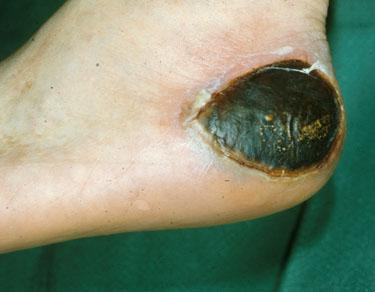
\includegraphics[width=0.7in]{dataset/dataset_3/luka_hitam/ready/2.jpg}&
		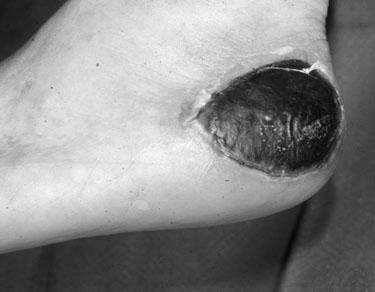
\includegraphics[width=0.7in]{dataset/dataset_3/luka_hitam/ready/2_gray.jpg}&
		375x292\\
		\hline
		
		& &  &  &\\
		2 & 
		luka\_hitam/4.jpg &
		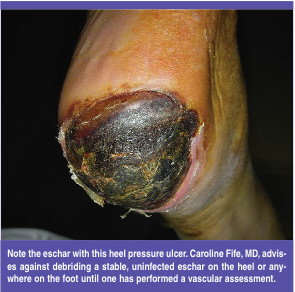
\includegraphics[width=0.7in]{dataset/dataset_3/luka_hitam/ready/4.jpg}&
		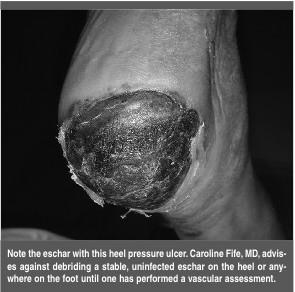
\includegraphics[width=0.7in]{dataset/dataset_3/luka_hitam/ready/4_gray.jpg}&
		295x292\\
		\hline
		
		& &  &  &\\
		3 & 
		luka\_hitam/5.jpg &
		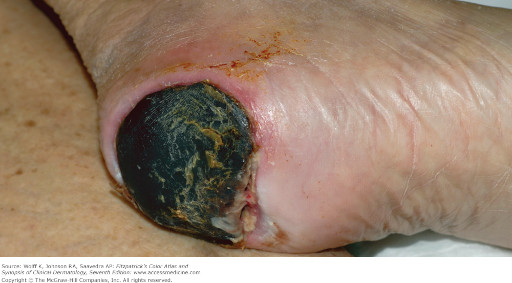
\includegraphics[width=0.7in]{dataset/dataset_3/luka_hitam/ready/5.jpg}&
		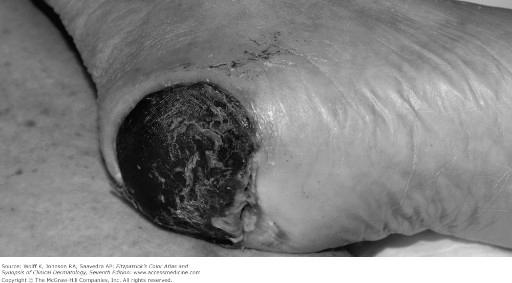
\includegraphics[width=0.7in]{dataset/dataset_3/luka_hitam/ready/5_gray.jpg}&
		512x283\\
		\hline
		
		& &  &  &\\
		4& 
		luka\_hitam/6.jpg &
		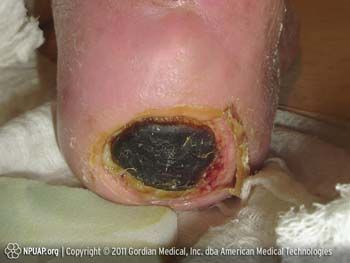
\includegraphics[width=0.7in]{dataset/dataset_3/luka_hitam/ready/6.jpg}&
		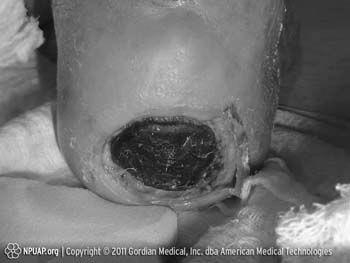
\includegraphics[width=0.7in]{dataset/dataset_3/luka_hitam/ready/6_gray.jpg}&
		350x263\\
		\hline
		
		& &  &  &\\
		5& 
		luka\_hitam/7.jpg &
		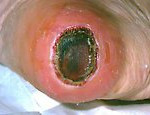
\includegraphics[width=0.7in]{dataset/dataset_3/luka_hitam/ready/7.jpg}&
		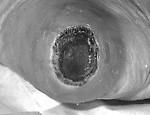
\includegraphics[width=0.7in]{dataset/dataset_3/luka_hitam/ready/7_gray.jpg}&
		150x115\\
		\hline
		
		& &  &  &\\
		6& 
		luka\_hitam/8.jpg &
		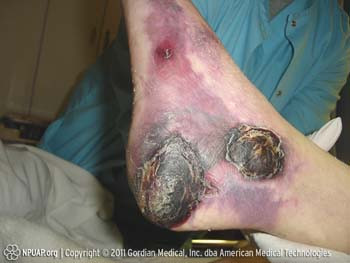
\includegraphics[width=0.7in]{dataset/dataset_3/luka_hitam/ready/8.jpg}&
		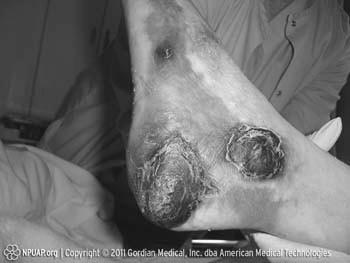
\includegraphics[width=0.7in]{dataset/dataset_3/luka_hitam/ready/8_gray.jpg}&
		350x263\\
		\hline
		
		& &  &  &\\
		7& 
		luka\_hitam/14.jpg &
		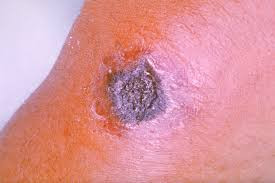
\includegraphics[width=0.7in]{dataset/dataset_3/luka_hitam/ready/14.jpg}&
		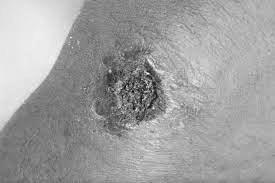
\includegraphics[width=0.7in]{dataset/dataset_3/luka_hitam/ready/14_gray.jpg}&
		275x183\\
		\hline
	\end{tabular}
\end{table}

\begin{table}[H]
	\centering
	\caption{Visualisasi hasil pengolahan data citra input luka hitam - lanjutan}
	\label{tabel_input_2}
	\begin{tabular}{|m{0.2in}|m{1.2in}|m{0.7in}|m{0.7in}|m{0.7in}|}
		\hline
		\textbf{No} & \textbf{File} & \textbf{Citra} & \textbf{\emph{grayscale}} & \textbf{resolusi} \\
		\hline
		
		& &  &  &\\
		8 & 
		luka\_hitam/15.jpg &
		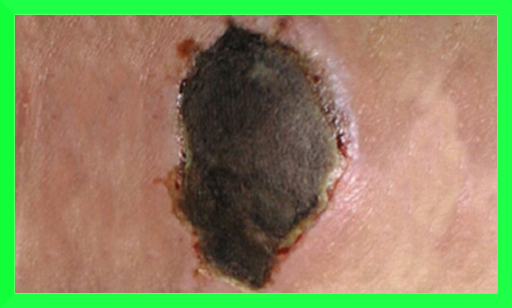
\includegraphics[width=0.7in]{dataset/dataset_3/luka_hitam/ready/15.jpg}&
		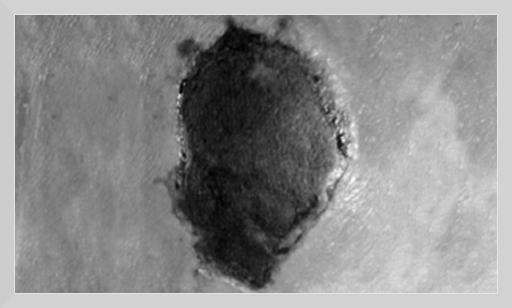
\includegraphics[width=0.7in]{dataset/dataset_3/luka_hitam/ready/15_gray.jpg}&
		512x308\\
		\hline
		
		& &  &  &\\
		9 & 
		luka\_hitam/17.jpg &
		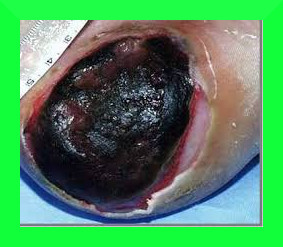
\includegraphics[width=0.7in]{dataset/dataset_3/luka_hitam/ready/17.jpg}&
		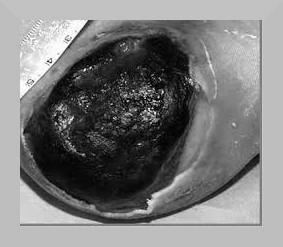
\includegraphics[width=0.7in]{dataset/dataset_3/luka_hitam/ready/17_gray.jpg}&
		283x247\\
		\hline
		
		& &  &  &\\
		10 & 
		luka\_hitam/18.jpg &
		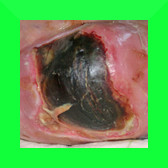
\includegraphics[width=0.7in]{dataset/dataset_3/luka_hitam/ready/18.jpg}&
		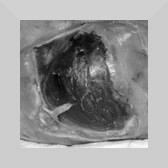
\includegraphics[width=0.7in]{dataset/dataset_3/luka_hitam/ready/18_gray.jpg}&
		168x168\\
		\hline
		
		& &  &  &\\
		11& 
		luka\_hitam/19.jpg &
		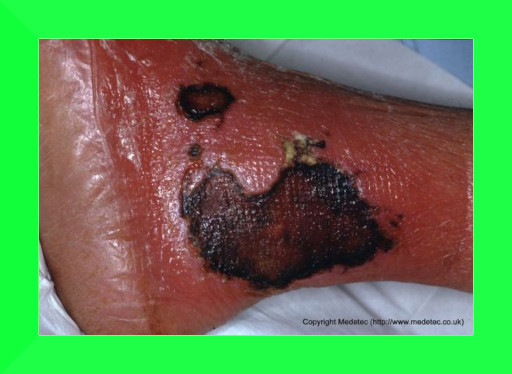
\includegraphics[width=0.7in]{dataset/dataset_3/luka_hitam/ready/19.jpg}&
		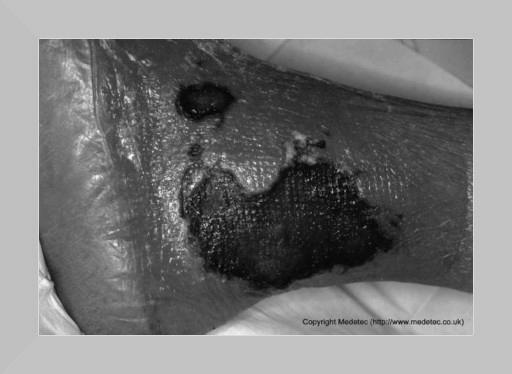
\includegraphics[width=0.7in]{dataset/dataset_3/luka_hitam/ready/19_gray.jpg}&
		512x374\\
		\hline
		
		& &  &  &\\
		12& 
		luka\_hitam/20.jpg &
		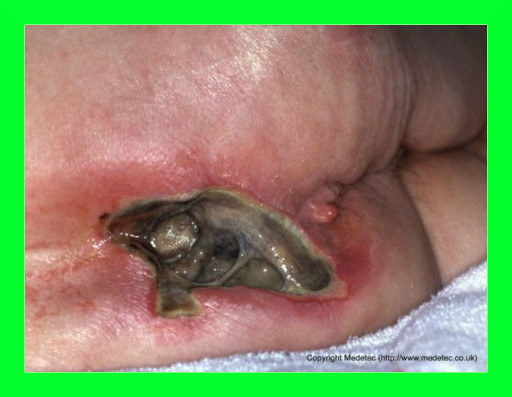
\includegraphics[width=0.7in]{dataset/dataset_3/luka_hitam/ready/20.jpg}&
		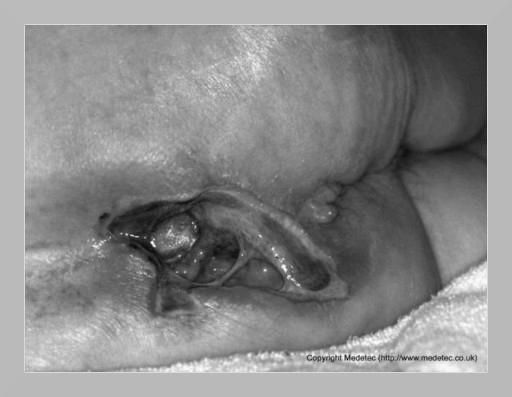
\includegraphics[width=0.7in]{dataset/dataset_3/luka_hitam/ready/20_gray.jpg}&
		512x397\\
		\hline
		
		& &  &  &\\
		13& 
		luka\_hitam/22.jpg &
		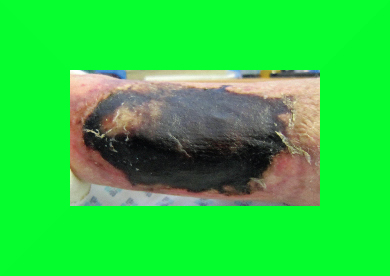
\includegraphics[width=0.7in]{dataset/dataset_3/luka_hitam/ready/22.jpg}&
		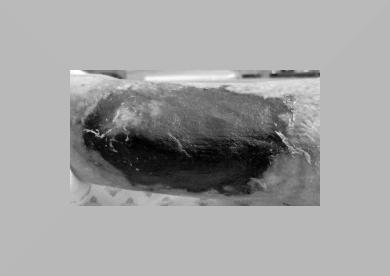
\includegraphics[width=0.7in]{dataset/dataset_3/luka_hitam/ready/22_gray.jpg}&
		390x276\\
		\hline
		
		& &  &  &\\
		14& 
		luka\_hitam/26.jpg &
		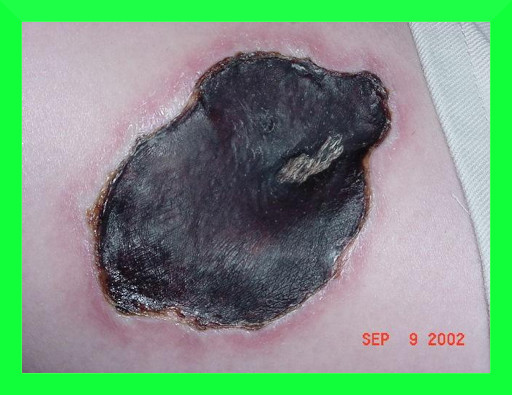
\includegraphics[width=0.7in]{dataset/dataset_3/luka_hitam/ready/26.jpg}&
		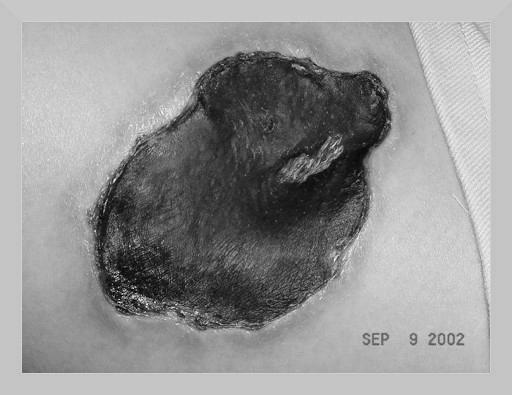
\includegraphics[width=0.7in]{dataset/dataset_3/luka_hitam/ready/26_gray.jpg}&
		512x395\\
		\hline
	\end{tabular}
\end{table}

\begin{table}[H]
	\centering
	\caption{Visualisasi hasil pengolahan data citra input luka hitam - lanjutan}
	\label{tabel_input_3}
	\begin{tabular}{|m{0.2in}|m{1.2in}|m{0.7in}|m{0.7in}|m{0.7in}|}
		\hline
		\textbf{No} & \textbf{File} & \textbf{Citra} & \textbf{\emph{grayscale}} & \textbf{resolusi} \\
		\hline
		
		& &  &  &\\
		15 & 
		luka\_hitam/27.jpg &
		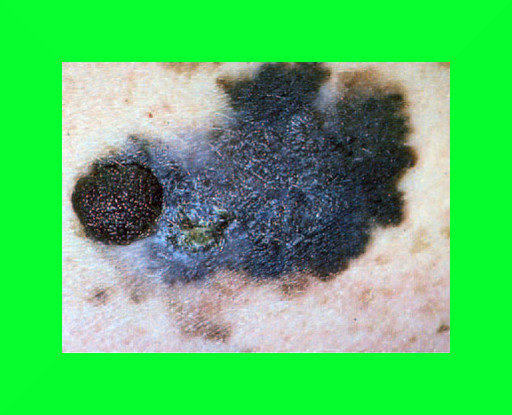
\includegraphics[width=0.7in]{dataset/dataset_3/luka_hitam/ready/27.jpg}&
		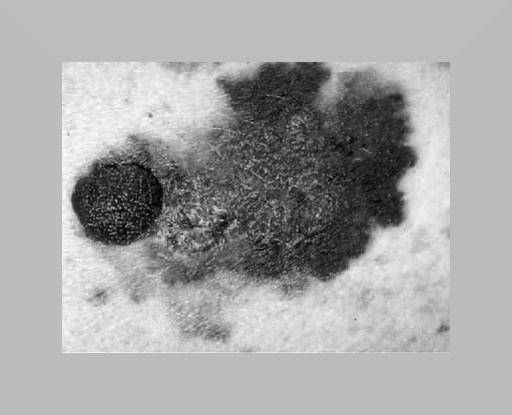
\includegraphics[width=0.7in]{dataset/dataset_3/luka_hitam/ready/27_gray.jpg}&
		512x415\\
		\hline
		
		& &  &  &\\
		16 & 
		luka\_hitam/28.jpg &
		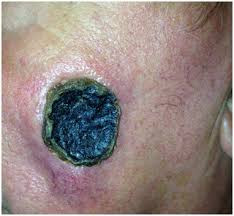
\includegraphics[width=0.7in]{dataset/dataset_3/luka_hitam/ready/28.jpg}&
		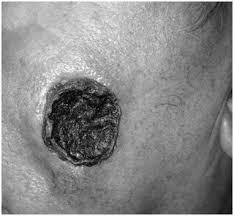
\includegraphics[width=0.7in]{dataset/dataset_3/luka_hitam/ready/28_gray.jpg}&
		234x216\\
		\hline
		
		& &  &  &\\
		17 & 
		luka\_hitam/29.jpg &
		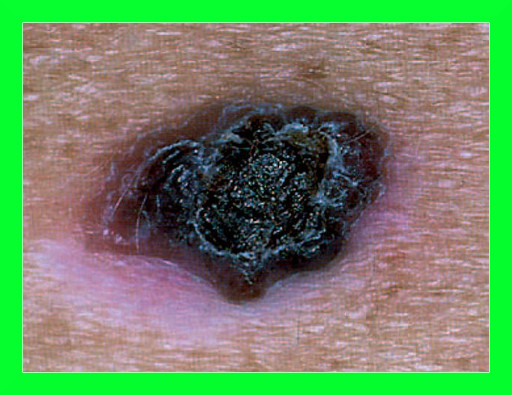
\includegraphics[width=0.7in]{dataset/dataset_3/luka_hitam/ready/29.jpg}&
		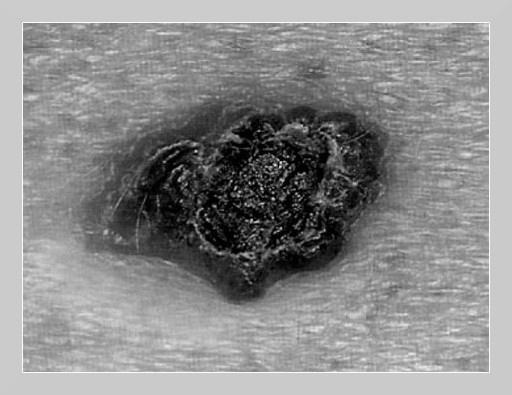
\includegraphics[width=0.7in]{dataset/dataset_3/luka_hitam/ready/29_gray.jpg}&
		512x395\\
		\hline
		
		& &  &  &\\
		18& 
		luka\_hitam/33.jpg &
		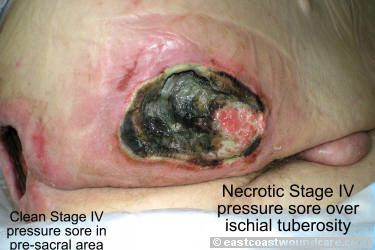
\includegraphics[width=0.7in]{dataset/dataset_3/luka_hitam/ready/33.jpg}&
		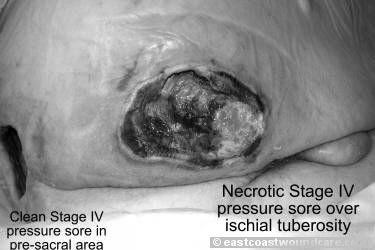
\includegraphics[width=0.7in]{dataset/dataset_3/luka_hitam/ready/33_gray.jpg}&
		375x250\\
		\hline
		
		& &  &  &\\
		19& 
		luka\_hitam/37.jpg &
		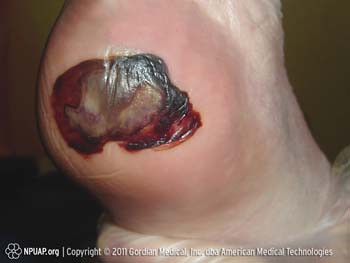
\includegraphics[width=0.7in]{dataset/dataset_3/luka_hitam/ready/37.jpg}&
		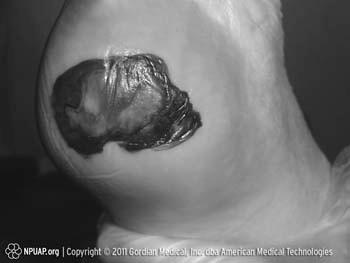
\includegraphics[width=0.7in]{dataset/dataset_3/luka_hitam/ready/37_gray.jpg}&
		350x263\\
		\hline
		
		& &  &  &\\
		20& 
		luka\_hitam/40.jpg &
		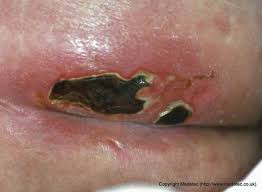
\includegraphics[width=0.7in]{dataset/dataset_3/luka_hitam/ready/40.jpg}&
		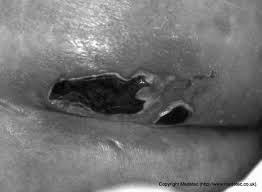
\includegraphics[width=0.7in]{dataset/dataset_3/luka_hitam/ready/40_gray.jpg}&
		262x192\\
		\hline
		
		& &  &  &\\
		21& 
		luka\_hitam/41.jpg &
		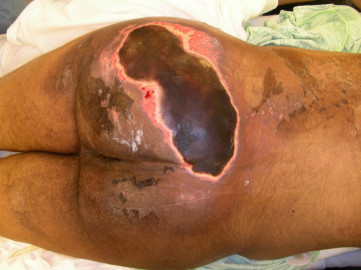
\includegraphics[width=0.7in]{dataset/dataset_3/luka_hitam/ready/41.jpg}&
		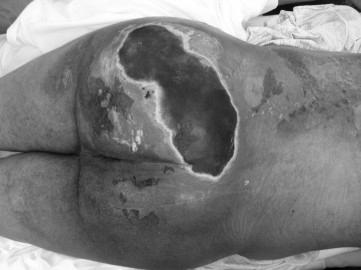
\includegraphics[width=0.7in]{dataset/dataset_3/luka_hitam/ready/41_gray.jpg}&
		361x270\\
		\hline
	\end{tabular}
\end{table}

\begin{table}[H]
	\centering
	\caption{Visualisasi hasil pengolahan data citra input luka hitam - lanjutan}
	\label{tabel_input_4}
	\begin{tabular}{|m{0.2in}|m{1.2in}|m{0.7in}|m{0.7in}|m{0.7in}|}
		\hline
		\textbf{No} & \textbf{File} & \textbf{Citra} & \textbf{\emph{grayscale}} & \textbf{resolusi} \\
		\hline
		
		& &  &  &\\
		22 & 
		luka\_hitam/16.jpg &
		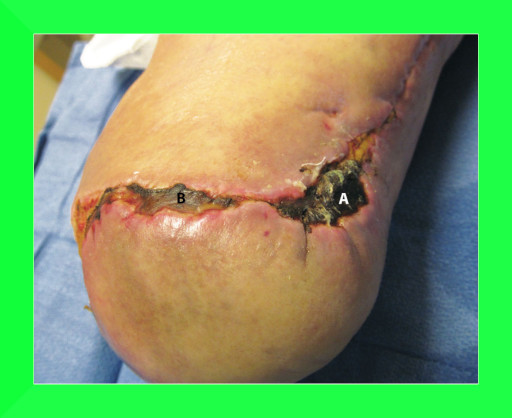
\includegraphics[width=0.7in]{dataset/dataset_3/luka_hitam/ready/16.jpg}&
		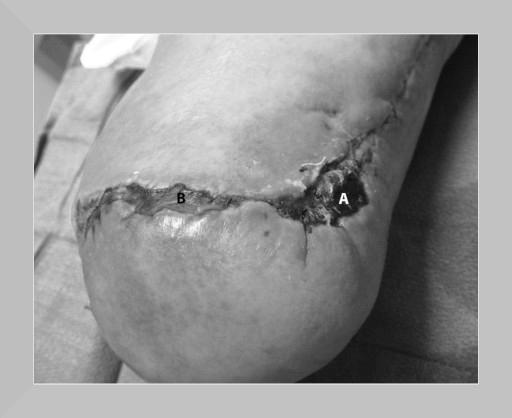
\includegraphics[width=0.7in]{dataset/dataset_3/luka_hitam/ready/16_gray.jpg}&
		512x418\\
		\hline
		
		& &  &  &\\
		23 & 
		luka\_hitam/31.jpg &
		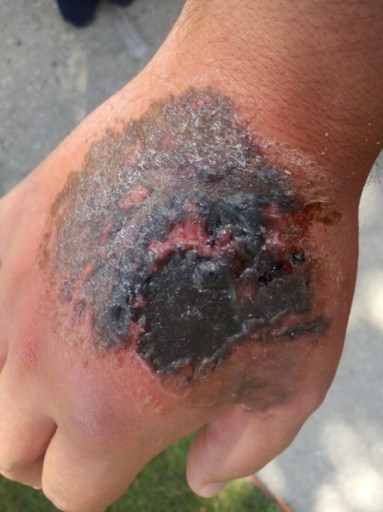
\includegraphics[width=0.7in]{dataset/dataset_3/luka_hitam/ready/31.jpg}&
		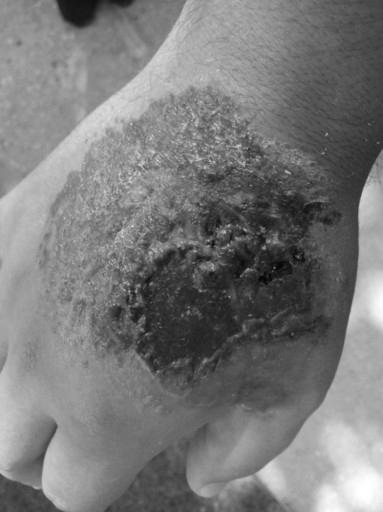
\includegraphics[width=0.7in]{dataset/dataset_3/luka_hitam/ready/31_gray.jpg}&
		383x512\\
		\hline
		
		& &  &  &\\
		24 & 
		luka\_hitam/39.jpg &
		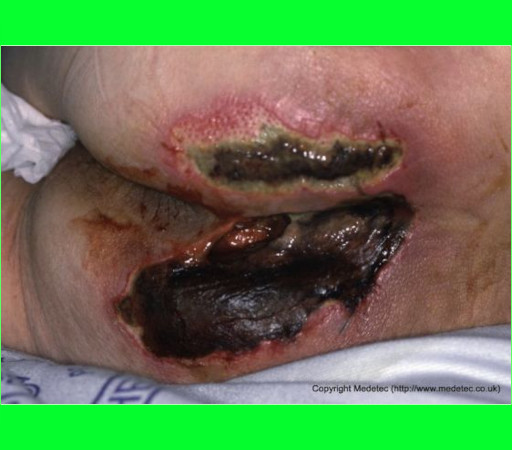
\includegraphics[width=0.7in]{dataset/dataset_3/luka_hitam/ready/39.jpg}&
		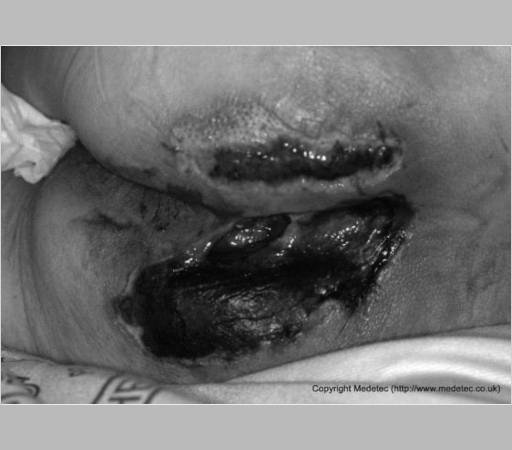
\includegraphics[width=0.7in]{dataset/dataset_3/luka_hitam/ready/39_gray.jpg}&
		512x450\\
		\hline
	\end{tabular}
\end{table}


\begin{table}[H]
	\centering
	\caption{Visualisasi hasil pengolahan data citra input luka kuning}
	\label{tabel_input_5}
	\begin{tabular}{|m{0.2in}|m{1.2in}|m{0.7in}|m{0.7in}|m{0.7in}|}
		\hline
		\textbf{No} & \textbf{File} & \textbf{Citra} & \textbf{\emph{grayscale}} & \textbf{resolusi} \\
		\hline
		
		& &  &  &\\
		1 & 
		luka\_kuning/13.jpg &
		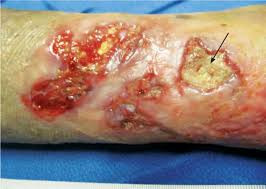
\includegraphics[width=0.7in]{dataset/dataset_3/luka_kuning/ready/13.jpg}&
		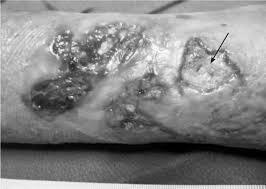
\includegraphics[width=0.7in]{dataset/dataset_3/luka_kuning/ready/13_gray.jpg}&
		266x189\\
		\hline
		
		& &  &  &\\
		2& 
		luka\_kuning/17.jpg &
		\includegraphics[width=0.7in]{dataset/dataset_3/luka_kuning/ready/17.jpg}&
		\includegraphics[width=0.7in]{dataset/dataset_3/luka_kuning/ready/17_gray.jpg}&
		259x194\\
		\hline
		
		& &  &  &\\
		3& 
		luka\_kuning/18.jpg &
		\includegraphics[width=0.7in]{dataset/dataset_3/luka_kuning/ready/18.jpg}&
		\includegraphics[width=0.7in]{dataset/dataset_3/luka_kuning/ready/18_gray.jpg}&
		265x190\\
		\hline
		
		& &  &  &\\
		4& 
		luka\_kuning/19.jpg &
		\includegraphics[width=0.7in]{dataset/dataset_3/luka_kuning/ready/19.jpg}&
		\includegraphics[width=0.7in]{dataset/dataset_3/luka_kuning/ready/19_gray.jpg}&
		120x151\\
		\hline
		
		& &  &  &\\
		5& 
		luka\_kuning/21.jpg &
		\includegraphics[width=0.7in]{dataset/dataset_3/luka_kuning/ready/21.jpg}&
		\includegraphics[width=0.7in]{dataset/dataset_3/luka_kuning/ready/21_gray.jpg}&
		357x242\\
		\hline
		
		& &  &  &\\
		6& 
		luka\_kuning/23.jpg &
		\includegraphics[width=0.7in]{dataset/dataset_3/luka_kuning/ready/23.jpg}&
		\includegraphics[width=0.7in]{dataset/dataset_3/luka_kuning/ready/23_gray.jpg}&
		500x333\\
		\hline
		
		& &  &  &\\
		7& 
		luka\_kuning/25.jpg &
		\includegraphics[width=0.7in]{dataset/dataset_3/luka_kuning/ready/25.jpg}&
		\includegraphics[width=0.7in]{dataset/dataset_3/luka_kuning/ready/25_gray.jpg}&
		288x216\\
		\hline
	\end{tabular}
\end{table}


\begin{table}[H]
	\centering
	\caption{Visualisasi hasil pengolahan data citra input luka kuning - lanjutan}
	\label{tabel_input_6}
	\begin{tabular}{|m{0.2in}|m{1.2in}|m{0.7in}|m{0.7in}|m{0.7in}|}
		\hline
		\textbf{No} & \textbf{File} & \textbf{Citra} & \textbf{\emph{grayscale}} & \textbf{resolusi} \\
		\hline
		
		& &  &  &\\
		8 & 
		luka\_kuning/34.jpg &
		\includegraphics[width=0.7in]{dataset/dataset_3/luka_kuning/ready/34.jpg}&
		\includegraphics[width=0.7in]{dataset/dataset_3/luka_kuning/ready/34_gray.jpg}&
		500x385\\
		\hline
		
		& &  &  &\\
		9& 
		luka\_kuning/35.jpg &
		\includegraphics[width=0.7in]{dataset/dataset_3/luka_kuning/ready/35.jpg}&
		\includegraphics[width=0.7in]{dataset/dataset_3/luka_kuning/ready/35_gray.jpg}&
		242x208\\
		\hline
		
		& &  &  &\\
		10& 
		luka\_kuning/38.jpg &
		\includegraphics[width=0.7in]{dataset/dataset_3/luka_kuning/ready/38.jpg}&
		\includegraphics[width=0.7in]{dataset/dataset_3/luka_kuning/ready/38_gray.jpg}&
		512x367\\
		\hline
		
		& &  &  &\\
		11& 
		luka\_kuning/42.jpg &
		\includegraphics[width=0.7in]{dataset/dataset_3/luka_kuning/ready/42.jpg}&
		\includegraphics[width=0.7in]{dataset/dataset_3/luka_kuning/ready/42_gray.jpg}&
		512x384\\
		\hline
		
		& &  &  &\\
		12& 
		luka\_kuning/3.jpg &
		\includegraphics[width=0.7in]{dataset/dataset_3/luka_kuning/ready/3.jpg}&
		\includegraphics[width=0.7in]{dataset/dataset_3/luka_kuning/ready/3_gray.jpg}&
		220x157\\
		\hline
		
		& &  &  &\\
		13& 
		luka\_kuning/12.jpg &
		\includegraphics[width=0.7in]{dataset/dataset_3/luka_kuning/ready/12.jpg}&
		\includegraphics[width=0.7in]{dataset/dataset_3/luka_kuning/ready/12_gray.jpg}&
		500x333\\
		\hline
		
		& &  &  &\\
		14& 
		luka\_kuning/10.jpg &
		\includegraphics[width=0.7in]{dataset/dataset_3/luka_kuning/ready/10.jpg}&
		\includegraphics[width=0.7in]{dataset/dataset_3/luka_kuning/ready/10_gray.jpg}&
		276x183\\
		\hline
	\end{tabular}
\end{table}

\begin{table}[H]
	\centering
	\caption{Visualisasi hasil pengolahan data citra input luka kuning - lanjutan}
	\label{tabel_input_7}
	\begin{tabular}{|m{0.2in}|m{1.2in}|m{0.7in}|m{0.7in}|m{0.7in}|}
		\hline
		\textbf{No} & \textbf{File} & \textbf{Citra} & \textbf{\emph{grayscale}} & \textbf{resolusi} \\
		\hline
		
		& &  &  &\\
		15 & 
		luka\_kuning/16.jpg &
		\includegraphics[width=0.7in]{dataset/dataset_3/luka_kuning/ready/16.jpg}&
		\includegraphics[width=0.7in]{dataset/dataset_3/luka_kuning/ready/16_gray.jpg}&
		346x270\\
		\hline
	\end{tabular}
\end{table}


\begin{table}[H]
	\centering
	\caption{Visualisasi hasil pengolahan data citra input luka merah}
	\label{tabel_input_8}
	\begin{tabular}{|m{0.2in}|m{1.2in}|m{0.7in}|m{0.7in}|m{0.7in}|}
		\hline
		\textbf{No} & \textbf{File} & \textbf{Citra} & \textbf{\emph{grayscale}} & \textbf{resolusi} \\
		\hline
		
		& &  &  &\\
		1 & 
		luka\_merah/16.jpg &
		\includegraphics[width=0.7in]{dataset/dataset_3/luka_merah/ready/16.jpg}&
		\includegraphics[width=0.7in]{dataset/dataset_3/luka_merah/ready/16_gray.jpg}&
		309x231\\
		\hline
		
		& &  &  &\\
		2& 
		luka\_merah/17.jpg &
		\includegraphics[width=0.7in]{dataset/dataset_3/luka_merah/ready/17.jpg}&
		\includegraphics[width=0.7in]{dataset/dataset_3/luka_merah/ready/17_gray.jpg}&
		328x218\\
		\hline
		
		& &  &  &\\
		3& 
		luka\_merah/22.jpg &
		\includegraphics[width=0.7in]{dataset/dataset_3/luka_merah/ready/22.jpg}&
		\includegraphics[width=0.7in]{dataset/dataset_3/luka_merah/ready/22_gray.jpg}&
		512x396\\
		\hline
		
		& &  &  &\\
		4& 
		luka\_merah/24.jpg &
		\includegraphics[width=0.7in]{dataset/dataset_3/luka_merah/ready/24.jpg}&
		\includegraphics[width=0.7in]{dataset/dataset_3/luka_merah/ready/24_gray.jpg}&
		302x308\\
		\hline
		
		& &  &  &\\
		5& 
		luka\_merah/25.jpg &
		\includegraphics[width=0.7in]{dataset/dataset_3/luka_merah/ready/25.jpg}&
		\includegraphics[width=0.7in]{dataset/dataset_3/luka_merah/ready/25_gray.jpg}&
		512x507\\
		\hline
		
		& &  &  &\\
		6& 
		luka\_merah/30.jpg &
		\includegraphics[width=0.7in]{dataset/dataset_3/luka_merah/ready/30.jpg}&
		\includegraphics[width=0.7in]{dataset/dataset_3/luka_merah/ready/30_gray.jpg}&
		260x194\\
		\hline
		
		& &  &  &\\
		7& 
		luka\_merah/32.jpg &
		\includegraphics[width=0.7in]{dataset/dataset_3/luka_merah/ready/32.jpg}&
		\includegraphics[width=0.7in]{dataset/dataset_3/luka_merah/ready/32_gray.jpg}&
		236x178\\
		\hline
	\end{tabular}
\end{table}

\begin{table}[H]
	\centering
	\caption{Visualisasi hasil pengolahan data citra input luka merah - lanjutan}
	\label{tabel_input_9}
	\begin{tabular}{|m{0.2in}|m{1.2in}|m{0.7in}|m{0.7in}|m{0.7in}|}
		\hline
		\textbf{No} & \textbf{File} & \textbf{Citra} & \textbf{\emph{grayscale}} & \textbf{resolusi} \\
		\hline
		
		& &  &  &\\
		8 & 
		luka\_merah/33.jpg &
		\includegraphics[width=0.7in]{dataset/dataset_3/luka_merah/ready/33.jpg}&
		\includegraphics[width=0.7in]{dataset/dataset_3/luka_merah/ready/33_gray.jpg}&
		226x223\\
		\hline
		
		& &  &  &\\
		9& 
		luka\_merah/37.jpg &
		\includegraphics[width=0.7in]{dataset/dataset_3/luka_merah/ready/37.jpg}&
		\includegraphics[width=0.7in]{dataset/dataset_3/luka_merah/ready/37_gray.jpg}&
		260x194\\
		\hline
		
		& &  &  &\\
		10& 
		luka\_merah/39.jpg &
		\includegraphics[width=0.7in]{dataset/dataset_3/luka_merah/ready/39.jpg}&
		\includegraphics[width=0.7in]{dataset/dataset_3/luka_merah/ready/39_gray.jpg}&
		185x139\\
		\hline
		
		& &  &  &\\
		11& 
		luka\_merah/42.jpg &
		\includegraphics[width=0.7in]{dataset/dataset_3/luka_merah/ready/42.jpg}&
		\includegraphics[width=0.7in]{dataset/dataset_3/luka_merah/ready/42_gray.jpg}&
		350x354\\
		\hline
		
		& &  &  &\\
		12& 
		luka\_merah/44.jpg &
		\includegraphics[width=0.7in]{dataset/dataset_3/luka_merah/ready/44.jpg}&
		\includegraphics[width=0.7in]{dataset/dataset_3/luka_merah/ready/44_gray.jpg}&
		512x363\\
		\hline
		
		& &  &  &\\
		13& 
		luka\_merah/2.jpg &
		\includegraphics[width=0.7in]{dataset/dataset_3/luka_merah/ready/2.jpg}&
		\includegraphics[width=0.7in]{dataset/dataset_3/luka_merah/ready/2_gray.jpg}&
		288x512\\
		\hline
		
		& &  &  &\\
		14& 
		luka\_merah/3.jpg &
		\includegraphics[width=0.7in]{dataset/dataset_3/luka_merah/ready/3.jpg}&
		\includegraphics[width=0.7in]{dataset/dataset_3/luka_merah/ready/3_gray.jpg}&
		384x512\\
		\hline
	\end{tabular}
\end{table}

\begin{table}[H]
	\centering
	\caption{Visualisasi hasil pengolahan data citra input luka merah - lanjutan}
	\label{tabel_input_10}
	\begin{tabular}{|m{0.2in}|m{1.2in}|m{0.7in}|m{0.7in}|m{0.7in}|}
		\hline
		\textbf{No} & \textbf{File} & \textbf{Citra} & \textbf{\emph{grayscale}} & \textbf{resolusi} \\
		\hline
		
		& &  &  &\\
		15 & 
		luka\_merah/4.jpg &
		\includegraphics[width=0.7in]{dataset/dataset_3/luka_merah/ready/4.jpg}&
		\includegraphics[width=0.7in]{dataset/dataset_3/luka_merah/ready/4_gray.jpg}&
		384x512\\
		\hline
		
		& &  &  &\\
		16& 
		luka\_merah/6.jpg &
		\includegraphics[width=0.7in]{dataset/dataset_3/luka_merah/ready/6.jpg}&
		\includegraphics[width=0.7in]{dataset/dataset_3/luka_merah/ready/6_gray.jpg}&
		512x384\\
		\hline
		
		& &  &  &\\
		17& 
		luka\_merah/7.jpg &
		\includegraphics[width=0.7in]{dataset/dataset_3/luka_merah/ready/7.jpg}&
		\includegraphics[width=0.7in]{dataset/dataset_3/luka_merah/ready/7_gray.jpg}&
		512x341\\
		\hline
		
		& &  &  &\\
		18& 
		luka\_merah/8.jpg &
		\includegraphics[width=0.7in]{dataset/dataset_3/luka_merah/ready/8.jpg}&
		\includegraphics[width=0.7in]{dataset/dataset_3/luka_merah/ready/8_gray.jpg}&
		512x384\\
		\hline
		
		& &  &  &\\
		19& 
		luka\_merah/9.jpg &
		\includegraphics[width=0.7in]{dataset/dataset_3/luka_merah/ready/9.jpg}&
		\includegraphics[width=0.7in]{dataset/dataset_3/luka_merah/ready/9_gray.jpg}&
		288x512\\
		\hline
		
		& &  &  &\\
		20& 
		luka\_merah/10.jpg &
		\includegraphics[width=0.7in]{dataset/dataset_3/luka_merah/ready/10.jpg}&
		\includegraphics[width=0.7in]{dataset/dataset_3/luka_merah/ready/10_gray.jpg}&
		512x384\\
		\hline
		
		& &  &  &\\
		21& 
		luka\_merah/11.jpg &
		\includegraphics[width=0.7in]{dataset/dataset_3/luka_merah/ready/11.jpg}&
		\includegraphics[width=0.7in]{dataset/dataset_3/luka_merah/ready/11_gray.jpg}&
		512x384\\
		\hline
	\end{tabular}
\end{table}

\begin{table}[H]
	\centering
	\caption{Visualisasi hasil pengolahan data citra input luka merah - lanjutan}
	\label{tabel_input_11}
	\begin{tabular}{|m{0.2in}|m{1.2in}|m{0.7in}|m{0.7in}|m{0.7in}|}
		\hline
		\textbf{No} & \textbf{File} & \textbf{Citra} & \textbf{\emph{grayscale}} & \textbf{resolusi} \\
		\hline
		
		& &  &  &\\
		22 & 
		luka\_merah/12.jpg &
		\includegraphics[width=0.7in]{dataset/dataset_3/luka_merah/ready/12.jpg}&
		\includegraphics[width=0.7in]{dataset/dataset_3/luka_merah/ready/12_gray.jpg}&
		512x384\\
		\hline
		
		& &  &  &\\
		23& 
		luka\_merah/14.jpg &
		\includegraphics[width=0.7in]{dataset/dataset_3/luka_merah/ready/14.jpg}&
		\includegraphics[width=0.7in]{dataset/dataset_3/luka_merah/ready/14_gray.jpg}&
		512x384\\
		\hline
		
		& &  &  &\\
		24& 
		luka\_merah/18.jpg &
		\includegraphics[width=0.7in]{dataset/dataset_3/luka_merah/ready/18.jpg}&
		\includegraphics[width=0.7in]{dataset/dataset_3/luka_merah/ready/18_gray.jpg}&
		512x382\\
		\hline
		
		& &  &  &\\
		25& 
		luka\_merah/19.jpg &
		\includegraphics[width=0.7in]{dataset/dataset_3/luka_merah/ready/19.jpg}&
		\includegraphics[width=0.7in]{dataset/dataset_3/luka_merah/ready/19_gray.jpg}&
		512x458\\
		\hline
		
		& &  &  &\\
		26& 
		luka\_merah/20.jpg &
		\includegraphics[width=0.7in]{dataset/dataset_3/luka_merah/ready/20.jpg}&
		\includegraphics[width=0.7in]{dataset/dataset_3/luka_merah/ready/20_gray.jpg}&
		408x360\\
		\hline
		
		& &  &  &\\
		27& 
		luka\_merah/23.jpg &
		\includegraphics[width=0.7in]{dataset/dataset_3/luka_merah/ready/23.jpg}&
		\includegraphics[width=0.7in]{dataset/dataset_3/luka_merah/ready/23_gray.jpg}&
		512x384\\
		\hline
		
		& &  &  &\\
		28& 
		luka\_merah/26.jpg &
		\includegraphics[width=0.7in]{dataset/dataset_3/luka_merah/ready/26.jpg}&
		\includegraphics[width=0.7in]{dataset/dataset_3/luka_merah/ready/26_gray.jpg}&
		512x464\\
		\hline
	\end{tabular}
\end{table}

\begin{table}[H]
	\centering
	\caption{Visualisasi hasil pengolahan data citra input luka merah - lanjutan}
	\label{tabel_input_12}
	\begin{tabular}{|m{0.2in}|m{1.2in}|m{0.7in}|m{0.7in}|m{0.7in}|}
		\hline
		\textbf{No} & \textbf{File} & \textbf{Citra} & \textbf{\emph{grayscale}} & \textbf{resolusi} \\
		\hline
		
		& &  &  &\\
		29 & 
		luka\_merah/29.jpg &
		\includegraphics[width=0.7in]{dataset/dataset_3/luka_merah/ready/29.jpg}&
		\includegraphics[width=0.7in]{dataset/dataset_3/luka_merah/ready/29_gray.jpg}&
		328x218\\
		\hline
		
		& &  &  &\\
		29& 
		luka\_merah/35.jpg &
		\includegraphics[width=0.7in]{dataset/dataset_3/luka_merah/ready/35.jpg}&
		\includegraphics[width=0.7in]{dataset/dataset_3/luka_merah/ready/35_gray.jpg}&
		261x295\\
		\hline
		
		& &  &  &\\
		30& 
		luka\_merah/36.jpg &
		\includegraphics[width=0.7in]{dataset/dataset_3/luka_merah/ready/36.jpg}&
		\includegraphics[width=0.7in]{dataset/dataset_3/luka_merah/ready/36_gray.jpg}&
		295x194\\
		\hline
		
		& &  &  &\\
		31& 
		luka\_merah/38.jpg &
		\includegraphics[width=0.7in]{dataset/dataset_3/luka_merah/ready/38.jpg}&
		\includegraphics[width=0.7in]{dataset/dataset_3/luka_merah/ready/38_gray.jpg}&
		512x384\\
		\hline
		
		& &  &  &\\
		32& 
		luka\_merah/20.jpg &
		\includegraphics[width=0.7in]{dataset/dataset_3/luka_merah/ready/20.jpg}&
		\includegraphics[width=0.7in]{dataset/dataset_3/luka_merah/ready/20_gray.jpg}&
		408x360\\
		\hline
	\end{tabular}
\end{table}


\chapter{Tabel hasil deteksi keliling luka menggunakan \emph{snake} versi \emph{integer}}
\begin{table}[H]
	\centering
	\caption{Visualisasi hasil deteksi keliling luka menggunakan \emph{snake} versi \emph{integer}}
	\label{tabel_hasil_1}
	\begin{tabular}{|m{0.7in}|m{0.7in}|m{0.7in}|m{0.7in}|m{0.7in}|m{0.7in}|m{0.7in}|}
		\hline
		\textbf{Inisialisasi} & \textbf{\emph{Eksternal}} & \textbf{kurva akhir} & \textbf{kurva akhir \& \emph{ground truth}}& \textbf{area ground truth} & \textbf{area kurva} & \textbf{Kategori} \\
		\hline
		
		&  &  & & & &  \\
		\includegraphics[width=0.7in]{dataset/dataset_3/luka_hitam/ready/5_integer_init.jpg}&
		\includegraphics[width=0.7in]{dataset/dataset_3/luka_hitam/ready/5_integer_ext.jpg}&
		\includegraphics[width=0.7in]{dataset/dataset_3/luka_hitam/ready/5_integer_result.jpg}&
		\includegraphics[width=0.7in]{dataset/dataset_3/luka_hitam/ready/5_gt_r_integer.jpg}&
		\includegraphics[width=0.7in]{dataset/dataset_3/luka_hitam/ready/5_r.jpg}&
		\includegraphics[width=0.7in]{dataset/dataset_3/luka_hitam/ready/5_integer_r.jpg}&
		berhasil\\
		\hline
		
		&  &  & & & &  \\
		\includegraphics[width=0.7in]{dataset/dataset_3/luka_hitam/ready/7_integer_init.jpg}&
		\includegraphics[width=0.7in]{dataset/dataset_3/luka_hitam/ready/7_integer_ext.jpg}&
		\includegraphics[width=0.7in]{dataset/dataset_3/luka_hitam/ready/7_integer_result.jpg}&
		\includegraphics[width=0.7in]{dataset/dataset_3/luka_hitam/ready/7_gt_r_integer.jpg}&
		\includegraphics[width=0.7in]{dataset/dataset_3/luka_hitam/ready/7_r.jpg}&
		\includegraphics[width=0.7in]{dataset/dataset_3/luka_hitam/ready/7_integer_r.jpg}&
		berhasil\\
		\hline
		
		&  &  & & & &  \\
		\includegraphics[width=0.7in]{dataset/dataset_3/luka_hitam/ready/8_integer_init.jpg}&
		\includegraphics[width=0.7in]{dataset/dataset_3/luka_hitam/ready/8_integer_ext.jpg}&
		\includegraphics[width=0.7in]{dataset/dataset_3/luka_hitam/ready/8_integer_result.jpg}&
		\includegraphics[width=0.7in]{dataset/dataset_3/luka_hitam/ready/8_gt_r_integer.jpg}&
		\includegraphics[width=0.7in]{dataset/dataset_3/luka_hitam/ready/8_r.jpg}&
		\includegraphics[width=0.7in]{dataset/dataset_3/luka_hitam/ready/8_integer_r.jpg}&
		berhasil\\
		\hline
		
		&  &  & & & &  \\
		\includegraphics[width=0.7in]{dataset/dataset_3/luka_hitam/ready/14_integer_init.jpg}&
		\includegraphics[width=0.7in]{dataset/dataset_3/luka_hitam/ready/14_integer_ext.jpg}&
		\includegraphics[width=0.7in]{dataset/dataset_3/luka_hitam/ready/14_integer_result.jpg}&
		\includegraphics[width=0.7in]{dataset/dataset_3/luka_hitam/ready/14_gt_r_integer.jpg}&
		\includegraphics[width=0.7in]{dataset/dataset_3/luka_hitam/ready/14_r.jpg}&
		\includegraphics[width=0.7in]{dataset/dataset_3/luka_hitam/ready/14_integer_r.jpg}&
		berhasil\\
		\hline
		
		&  &  & & & &  \\
		\includegraphics[width=0.7in]{dataset/dataset_3/luka_hitam/ready/28_integer_init.jpg}&
		\includegraphics[width=0.7in]{dataset/dataset_3/luka_hitam/ready/28_integer_ext.jpg}&
		\includegraphics[width=0.7in]{dataset/dataset_3/luka_hitam/ready/28_integer_result.jpg}&
		\includegraphics[width=0.7in]{dataset/dataset_3/luka_hitam/ready/28_gt_r_integer.jpg}&
		\includegraphics[width=0.7in]{dataset/dataset_3/luka_hitam/ready/28_r.jpg}&
		\includegraphics[width=0.7in]{dataset/dataset_3/luka_hitam/ready/28_integer_r.jpg}&
		berhasil\\
		\hline
		
		&  &  & & & &  \\
		\includegraphics[width=0.7in]{dataset/dataset_3/luka_hitam/ready/2_integer_init.jpg}&
		\includegraphics[width=0.7in]{dataset/dataset_3/luka_hitam/ready/2_integer_ext.jpg}&
		\includegraphics[width=0.7in]{dataset/dataset_3/luka_hitam/ready/2_integer_result.jpg}&
		\includegraphics[width=0.7in]{dataset/dataset_3/luka_hitam/ready/2_gt_r_integer.jpg}&
		\includegraphics[width=0.7in]{dataset/dataset_3/luka_hitam/ready/2_r.jpg}&
		\includegraphics[width=0.7in]{dataset/dataset_3/luka_hitam/ready/2_integer_r.jpg}&
		gagal\\
		\hline
		
		&  &  & & & &  \\
		\includegraphics[width=0.7in]{dataset/dataset_3/luka_hitam/ready/4_integer_init.jpg}&
		\includegraphics[width=0.7in]{dataset/dataset_3/luka_hitam/ready/4_integer_ext.jpg}&
		\includegraphics[width=0.7in]{dataset/dataset_3/luka_hitam/ready/4_integer_result.jpg}&
		\includegraphics[width=0.7in]{dataset/dataset_3/luka_hitam/ready/4_gt_r_integer.jpg}&
		\includegraphics[width=0.7in]{dataset/dataset_3/luka_hitam/ready/4_r.jpg}&
		\includegraphics[width=0.7in]{dataset/dataset_3/luka_hitam/ready/4_integer_r.jpg}&
		gagal\\
		\hline
		
	\end{tabular}
\end{table}

\begin{table}[H]
	\centering
	\caption{Visualisasi hasil deteksi keliling luka menggunakan \emph{snake} versi \emph{integer} - lanjutan}
	\label{tabel_hasil_2}
	\begin{tabular}{|m{0.7in}|m{0.7in}|m{0.7in}|m{0.7in}|m{0.7in}|m{0.7in}|m{0.7in}|}
		\hline
		\textbf{Inisialisasi} & \textbf{\emph{Eksternal}} & \textbf{kurva akhir} & \textbf{kurva akhir \& \emph{ground truth}}& \textbf{area ground truth} & \textbf{area kurva} & \textbf{Kategori} \\
		\hline
		
		&  &  & & & &  \\
		\includegraphics[width=0.7in]{dataset/dataset_3/luka_hitam/ready/6_integer_init.jpg}&
		\includegraphics[width=0.7in]{dataset/dataset_3/luka_hitam/ready/6_integer_ext.jpg}&
		\includegraphics[width=0.7in]{dataset/dataset_3/luka_hitam/ready/6_integer_result.jpg}&
		\includegraphics[width=0.7in]{dataset/dataset_3/luka_hitam/ready/6_gt_r_integer.jpg}&
		\includegraphics[width=0.7in]{dataset/dataset_3/luka_hitam/ready/6_r.jpg}&
		\includegraphics[width=0.7in]{dataset/dataset_3/luka_hitam/ready/6_integer_r.jpg}&
		gagal\\
		\hline
		
		&  &  & & & &  \\
		\includegraphics[width=0.7in]{dataset/dataset_3/luka_hitam/ready/15_integer_init.jpg}&
		\includegraphics[width=0.7in]{dataset/dataset_3/luka_hitam/ready/15_integer_ext.jpg}&
		\includegraphics[width=0.7in]{dataset/dataset_3/luka_hitam/ready/15_integer_result.jpg}&
		\includegraphics[width=0.7in]{dataset/dataset_3/luka_hitam/ready/15_gt_r_integer.jpg}&
		\includegraphics[width=0.7in]{dataset/dataset_3/luka_hitam/ready/15_r.jpg}&
		\includegraphics[width=0.7in]{dataset/dataset_3/luka_hitam/ready/15_integer_r.jpg}&
		gagal\\
		\hline
		
		&  &  & & & &  \\
		\includegraphics[width=0.7in]{dataset/dataset_3/luka_hitam/ready/16_integer_init.jpg}&
		\includegraphics[width=0.7in]{dataset/dataset_3/luka_hitam/ready/16_integer_ext.jpg}&
		\includegraphics[width=0.7in]{dataset/dataset_3/luka_hitam/ready/16_integer_result.jpg}&
		\includegraphics[width=0.7in]{dataset/dataset_3/luka_hitam/ready/16_gt_r_integer.jpg}&
		\includegraphics[width=0.7in]{dataset/dataset_3/luka_hitam/ready/16_r.jpg}&
		\includegraphics[width=0.7in]{dataset/dataset_3/luka_hitam/ready/16_integer_r.jpg}&
		gagal\\
		\hline
		
		&  &  & & & &  \\
		\includegraphics[width=0.7in]{dataset/dataset_3/luka_hitam/ready/17_integer_init.jpg}&
		\includegraphics[width=0.7in]{dataset/dataset_3/luka_hitam/ready/17_integer_ext.jpg}&
		\includegraphics[width=0.7in]{dataset/dataset_3/luka_hitam/ready/17_integer_result.jpg}&
		\includegraphics[width=0.7in]{dataset/dataset_3/luka_hitam/ready/17_gt_r_integer.jpg}&
		\includegraphics[width=0.7in]{dataset/dataset_3/luka_hitam/ready/17_r.jpg}&
		\includegraphics[width=0.7in]{dataset/dataset_3/luka_hitam/ready/17_integer_r.jpg}&
		gagal\\
		\hline
		
		&  &  & & & &  \\
		\includegraphics[width=0.7in]{dataset/dataset_3/luka_hitam/ready/18_integer_init.jpg}&
		\includegraphics[width=0.7in]{dataset/dataset_3/luka_hitam/ready/18_integer_ext.jpg}&
		\includegraphics[width=0.7in]{dataset/dataset_3/luka_hitam/ready/18_integer_result.jpg}&
		\includegraphics[width=0.7in]{dataset/dataset_3/luka_hitam/ready/18_gt_r_integer.jpg}&
		\includegraphics[width=0.7in]{dataset/dataset_3/luka_hitam/ready/18_r.jpg}&
		\includegraphics[width=0.7in]{dataset/dataset_3/luka_hitam/ready/18_integer_r.jpg}&
		gagal\\
		\hline
		
		&  &  & & & &  \\
		\includegraphics[width=0.7in]{dataset/dataset_3/luka_hitam/ready/19_integer_init.jpg}&
		\includegraphics[width=0.7in]{dataset/dataset_3/luka_hitam/ready/19_integer_ext.jpg}&
		\includegraphics[width=0.7in]{dataset/dataset_3/luka_hitam/ready/19_integer_result.jpg}&
		\includegraphics[width=0.7in]{dataset/dataset_3/luka_hitam/ready/19_gt_r_integer.jpg}&
		\includegraphics[width=0.7in]{dataset/dataset_3/luka_hitam/ready/19_r.jpg}&
		\includegraphics[width=0.7in]{dataset/dataset_3/luka_hitam/ready/19_integer_r.jpg}&
		gagal\\
		\hline
		
		&  &  & & & &  \\
		\includegraphics[width=0.7in]{dataset/dataset_3/luka_hitam/ready/20_integer_init.jpg}&
		\includegraphics[width=0.7in]{dataset/dataset_3/luka_hitam/ready/20_integer_ext.jpg}&
		\includegraphics[width=0.7in]{dataset/dataset_3/luka_hitam/ready/20_integer_result.jpg}&
		\includegraphics[width=0.7in]{dataset/dataset_3/luka_hitam/ready/20_gt_r_integer.jpg}&
		\includegraphics[width=0.7in]{dataset/dataset_3/luka_hitam/ready/20_r.jpg}&
		\includegraphics[width=0.7in]{dataset/dataset_3/luka_hitam/ready/20_integer_r.jpg}&
		gagal\\
		\hline
		
	\end{tabular}
\end{table}

\begin{table}[H]
	\centering
	\caption{Visualisasi hasil deteksi keliling luka menggunakan \emph{snake} versi \emph{integer} - lanjutan}
	\label{tabel_hasil_3}
	\begin{tabular}{|m{0.7in}|m{0.7in}|m{0.7in}|m{0.7in}|m{0.7in}|m{0.7in}|m{0.7in}|}
		\hline
		\textbf{Inisialisasi} & \textbf{\emph{Eksternal}} & \textbf{kurva akhir} & \textbf{kurva akhir \& \emph{ground truth}}& \textbf{area ground truth} & \textbf{area kurva} & \textbf{Kategori} \\
		\hline
		
		&  &  & & & &  \\
		\includegraphics[width=0.7in]{dataset/dataset_3/luka_hitam/ready/22_integer_init.jpg}&
		\includegraphics[width=0.7in]{dataset/dataset_3/luka_hitam/ready/22_integer_ext.jpg}&
		\includegraphics[width=0.7in]{dataset/dataset_3/luka_hitam/ready/22_integer_result.jpg}&
		\includegraphics[width=0.7in]{dataset/dataset_3/luka_hitam/ready/22_gt_r_integer.jpg}&
		\includegraphics[width=0.7in]{dataset/dataset_3/luka_hitam/ready/22_r.jpg}&
		\includegraphics[width=0.7in]{dataset/dataset_3/luka_hitam/ready/22_integer_r.jpg}&
		gagal\\
		\hline
		
		&  &  & & & &  \\
		\includegraphics[width=0.7in]{dataset/dataset_3/luka_hitam/ready/26_integer_init.jpg}&
		\includegraphics[width=0.7in]{dataset/dataset_3/luka_hitam/ready/26_integer_ext.jpg}&
		\includegraphics[width=0.7in]{dataset/dataset_3/luka_hitam/ready/26_integer_result.jpg}&
		\includegraphics[width=0.7in]{dataset/dataset_3/luka_hitam/ready/26_gt_r_integer.jpg}&
		\includegraphics[width=0.7in]{dataset/dataset_3/luka_hitam/ready/26_r.jpg}&
		\includegraphics[width=0.7in]{dataset/dataset_3/luka_hitam/ready/26_integer_r.jpg}&
		gagal\\
		\hline
		
		&  &  & & & &  \\
		\includegraphics[width=0.7in]{dataset/dataset_3/luka_hitam/ready/27_integer_init.jpg}&
		\includegraphics[width=0.7in]{dataset/dataset_3/luka_hitam/ready/27_integer_ext.jpg}&
		\includegraphics[width=0.7in]{dataset/dataset_3/luka_hitam/ready/27_integer_result.jpg}&
		\includegraphics[width=0.7in]{dataset/dataset_3/luka_hitam/ready/27_gt_r_integer.jpg}&
		\includegraphics[width=0.7in]{dataset/dataset_3/luka_hitam/ready/27_r.jpg}&
		\includegraphics[width=0.7in]{dataset/dataset_3/luka_hitam/ready/27_integer_r.jpg}&
		gagal\\
		\hline
		
		&  &  & & & &  \\
		\includegraphics[width=0.7in]{dataset/dataset_3/luka_hitam/ready/29_integer_init.jpg}&
		\includegraphics[width=0.7in]{dataset/dataset_3/luka_hitam/ready/29_integer_ext.jpg}&
		\includegraphics[width=0.7in]{dataset/dataset_3/luka_hitam/ready/29_integer_result.jpg}&
		\includegraphics[width=0.7in]{dataset/dataset_3/luka_hitam/ready/29_gt_r_integer.jpg}&
		\includegraphics[width=0.7in]{dataset/dataset_3/luka_hitam/ready/29_r.jpg}&
		\includegraphics[width=0.7in]{dataset/dataset_3/luka_hitam/ready/29_integer_r.jpg}&
		gagal\\
		\hline
		
		&  &  & & & &  \\
		\includegraphics[width=0.7in]{dataset/dataset_3/luka_hitam/ready/31_integer_init.jpg}&
		\includegraphics[width=0.7in]{dataset/dataset_3/luka_hitam/ready/31_integer_ext.jpg}&
		\includegraphics[width=0.7in]{dataset/dataset_3/luka_hitam/ready/31_integer_result.jpg}&
		\includegraphics[width=0.7in]{dataset/dataset_3/luka_hitam/ready/31_gt_r_integer.jpg}&
		\includegraphics[width=0.7in]{dataset/dataset_3/luka_hitam/ready/31_r.jpg}&
		\includegraphics[width=0.7in]{dataset/dataset_3/luka_hitam/ready/31_integer_r.jpg}&
		gagal\\
		\hline
		
		&  &  & & & &  \\
		\includegraphics[width=0.7in]{dataset/dataset_3/luka_hitam/ready/33_integer_init.jpg}&
		\includegraphics[width=0.7in]{dataset/dataset_3/luka_hitam/ready/33_integer_ext.jpg}&
		\includegraphics[width=0.7in]{dataset/dataset_3/luka_hitam/ready/33_integer_result.jpg}&
		\includegraphics[width=0.7in]{dataset/dataset_3/luka_hitam/ready/33_gt_r_integer.jpg}&
		\includegraphics[width=0.7in]{dataset/dataset_3/luka_hitam/ready/33_r.jpg}&
		\includegraphics[width=0.7in]{dataset/dataset_3/luka_hitam/ready/33_integer_r.jpg}&
		gagal\\
		\hline
		
		&  &  & & & &  \\
		\includegraphics[width=0.7in]{dataset/dataset_3/luka_hitam/ready/37_integer_init.jpg}&
		\includegraphics[width=0.7in]{dataset/dataset_3/luka_hitam/ready/37_integer_ext.jpg}&
		\includegraphics[width=0.7in]{dataset/dataset_3/luka_hitam/ready/37_integer_result.jpg}&
		\includegraphics[width=0.7in]{dataset/dataset_3/luka_hitam/ready/37_gt_r_integer.jpg}&
		\includegraphics[width=0.7in]{dataset/dataset_3/luka_hitam/ready/37_r.jpg}&
		\includegraphics[width=0.7in]{dataset/dataset_3/luka_hitam/ready/37_integer_r.jpg}&
		gagal\\
		\hline
		
	\end{tabular}
\end{table}

\begin{table}[H]
	\centering
	\caption{Visualisasi hasil deteksi keliling luka menggunakan \emph{snake} versi \emph{integer} - lanjutan}
	\label{tabel_hasil_4}
	\begin{tabular}{|m{0.7in}|m{0.7in}|m{0.7in}|m{0.7in}|m{0.7in}|m{0.7in}|m{0.7in}|}
		\hline
		\textbf{Inisialisasi} & \textbf{\emph{Eksternal}} & \textbf{kurva akhir} & \textbf{kurva akhir \& \emph{ground truth}}& \textbf{area ground truth} & \textbf{area kurva} & \textbf{Kategori} \\
		\hline
		
		&  &  & & & &  \\
		\includegraphics[width=0.7in]{dataset/dataset_3/luka_kuning/ready/13_integer_init.jpg}&
		\includegraphics[width=0.7in]{dataset/dataset_3/luka_kuning/ready/13_integer_ext.jpg}&
		\includegraphics[width=0.7in]{dataset/dataset_3/luka_kuning/ready/13_integer_result.jpg}&
		\includegraphics[width=0.7in]{dataset/dataset_3/luka_kuning/ready/13_gt_r_integer.jpg}&
		\includegraphics[width=0.7in]{dataset/dataset_3/luka_kuning/ready/13_r.jpg}&
		\includegraphics[width=0.7in]{dataset/dataset_3/luka_kuning/ready/13_integer_r.jpg}&
		berhasil\\
		\hline
		
		&  &  & & & &  \\
		\includegraphics[width=0.7in]{dataset/dataset_3/luka_kuning/ready/19_integer_init.jpg}&
		\includegraphics[width=0.7in]{dataset/dataset_3/luka_kuning/ready/19_integer_ext.jpg}&
		\includegraphics[width=0.7in]{dataset/dataset_3/luka_kuning/ready/19_integer_result.jpg}&
		\includegraphics[width=0.7in]{dataset/dataset_3/luka_kuning/ready/19_gt_r_integer.jpg}&
		\includegraphics[width=0.7in]{dataset/dataset_3/luka_kuning/ready/19_r.jpg}&
		\includegraphics[width=0.7in]{dataset/dataset_3/luka_kuning/ready/19_integer_r.jpg}&
		berhasil\\
		\hline
		
		&  &  & & & &  \\
		\includegraphics[width=0.7in]{dataset/dataset_3/luka_kuning/ready/21_integer_init.jpg}&
		\includegraphics[width=0.7in]{dataset/dataset_3/luka_kuning/ready/21_integer_ext.jpg}&
		\includegraphics[width=0.7in]{dataset/dataset_3/luka_kuning/ready/21_integer_result.jpg}&
		\includegraphics[width=0.7in]{dataset/dataset_3/luka_kuning/ready/21_gt_r_integer.jpg}&
		\includegraphics[width=0.7in]{dataset/dataset_3/luka_kuning/ready/21_r.jpg}&
		\includegraphics[width=0.7in]{dataset/dataset_3/luka_kuning/ready/21_integer_r.jpg}&
		berhasil\\
		\hline
		
		&  &  & & & &  \\
		\includegraphics[width=0.7in]{dataset/dataset_3/luka_kuning/ready/25_integer_init.jpg}&
		\includegraphics[width=0.7in]{dataset/dataset_3/luka_kuning/ready/25_integer_ext.jpg}&
		\includegraphics[width=0.7in]{dataset/dataset_3/luka_kuning/ready/25_integer_result.jpg}&
		\includegraphics[width=0.7in]{dataset/dataset_3/luka_kuning/ready/25_gt_r_integer.jpg}&
		\includegraphics[width=0.7in]{dataset/dataset_3/luka_kuning/ready/25_r.jpg}&
		\includegraphics[width=0.7in]{dataset/dataset_3/luka_kuning/ready/25_integer_r.jpg}&
		berhasil\\
		\hline
		
		
		&  &  & & & &  \\
		\includegraphics[width=0.7in]{dataset/dataset_3/luka_kuning/ready/34_integer_init.jpg}&
		\includegraphics[width=0.7in]{dataset/dataset_3/luka_kuning/ready/34_integer_ext.jpg}&
		\includegraphics[width=0.7in]{dataset/dataset_3/luka_kuning/ready/34_integer_result.jpg}&
		\includegraphics[width=0.7in]{dataset/dataset_3/luka_kuning/ready/34_gt_r_integer.jpg}&
		\includegraphics[width=0.7in]{dataset/dataset_3/luka_kuning/ready/34_r.jpg}&
		\includegraphics[width=0.7in]{dataset/dataset_3/luka_kuning/ready/34_integer_r.jpg}&
		berhasil \\
		\hline
		
		&  &  & & & &  \\
		\includegraphics[width=0.7in]{dataset/dataset_3/luka_kuning/ready/3_integer_init.jpg}&
		\includegraphics[width=0.7in]{dataset/dataset_3/luka_kuning/ready/3_integer_ext.jpg}&
		\includegraphics[width=0.7in]{dataset/dataset_3/luka_kuning/ready/3_integer_result.jpg}&
		\includegraphics[width=0.7in]{dataset/dataset_3/luka_kuning/ready/3_gt_r_integer.jpg}&
		\includegraphics[width=0.7in]{dataset/dataset_3/luka_kuning/ready/3_r.jpg}&
		\includegraphics[width=0.7in]{dataset/dataset_3/luka_kuning/ready/3_integer_r.jpg}&
		gagal\\
		\hline
		
		&  &  & & & &  \\
		\includegraphics[width=0.7in]{dataset/dataset_3/luka_kuning/ready/10_integer_init.jpg}&
		\includegraphics[width=0.7in]{dataset/dataset_3/luka_kuning/ready/10_integer_ext.jpg}&
		\includegraphics[width=0.7in]{dataset/dataset_3/luka_kuning/ready/10_integer_result.jpg}&
		\includegraphics[width=0.7in]{dataset/dataset_3/luka_kuning/ready/10_gt_r_integer.jpg}&
		\includegraphics[width=0.7in]{dataset/dataset_3/luka_kuning/ready/10_r.jpg}&
		\includegraphics[width=0.7in]{dataset/dataset_3/luka_kuning/ready/10_integer_r.jpg}&
		gagal\\
		\hline
	\end{tabular}
\end{table}

\begin{table}[H]
	\centering
	\caption{Visualisasi hasil deteksi keliling luka menggunakan \emph{snake} versi \emph{integer} - lanjutan}
	\label{tabel_hasil_45}
	\begin{tabular}{|m{0.7in}|m{0.7in}|m{0.7in}|m{0.7in}|m{0.7in}|m{0.7in}|m{0.7in}|}
		\hline
		\textbf{Inisialisasi} & \textbf{\emph{Eksternal}} & \textbf{kurva akhir} & \textbf{kurva akhir \& \emph{ground truth}}& \textbf{area ground truth} & \textbf{area kurva} & \textbf{Kategori} \\
		\hline
		
		&  &  & & & &  \\
		\includegraphics[width=0.7in]{dataset/dataset_3/luka_kuning/ready/12_integer_init.jpg}&
		\includegraphics[width=0.7in]{dataset/dataset_3/luka_kuning/ready/12_integer_ext.jpg}&
		\includegraphics[width=0.7in]{dataset/dataset_3/luka_kuning/ready/12_integer_result.jpg}&
		\includegraphics[width=0.7in]{dataset/dataset_3/luka_kuning/ready/12_gt_r_integer.jpg}&
		\includegraphics[width=0.7in]{dataset/dataset_3/luka_kuning/ready/12_r.jpg}&
		\includegraphics[width=0.7in]{dataset/dataset_3/luka_kuning/ready/12_integer_r.jpg}&
		gagal\\
		\hline
		
	\end{tabular}
\end{table}

\begin{table}[H]
	\centering
	\caption{Visualisasi hasil deteksi keliling luka menggunakan \emph{snake} versi \emph{integer} - lanjutan}
	\label{tabel_hasil_5}
	\begin{tabular}{|m{0.7in}|m{0.7in}|m{0.7in}|m{0.7in}|m{0.7in}|m{0.7in}|m{0.7in}|}
		\hline
		\textbf{Inisialisasi} & \textbf{\emph{Eksternal}} & \textbf{kurva akhir} & \textbf{kurva akhir \& \emph{ground truth}}& \textbf{area ground truth} & \textbf{area kurva} & \textbf{Kategori} \\
		\hline
		
		&  &  & & & &  \\
		\includegraphics[width=0.7in]{dataset/dataset_3/luka_kuning/ready/16_integer_init.jpg}&
		\includegraphics[width=0.7in]{dataset/dataset_3/luka_kuning/ready/16_integer_ext.jpg}&
		\includegraphics[width=0.7in]{dataset/dataset_3/luka_kuning/ready/16_integer_result.jpg}&
		\includegraphics[width=0.7in]{dataset/dataset_3/luka_kuning/ready/16_gt_r_integer.jpg}&
		\includegraphics[width=0.7in]{dataset/dataset_3/luka_kuning/ready/16_r.jpg}&
		\includegraphics[width=0.7in]{dataset/dataset_3/luka_kuning/ready/16_integer_r.jpg}&
		gagal\\
		\hline
		
		&  &  & & & &  \\
		\includegraphics[width=0.7in]{dataset/dataset_3/luka_kuning/ready/17_integer_init.jpg}&
		\includegraphics[width=0.7in]{dataset/dataset_3/luka_kuning/ready/17_integer_ext.jpg}&
		\includegraphics[width=0.7in]{dataset/dataset_3/luka_kuning/ready/17_integer_result.jpg}&
		\includegraphics[width=0.7in]{dataset/dataset_3/luka_kuning/ready/17_gt_r_integer.jpg}&
		\includegraphics[width=0.7in]{dataset/dataset_3/luka_kuning/ready/17_r.jpg}&
		\includegraphics[width=0.7in]{dataset/dataset_3/luka_kuning/ready/17_integer_r.jpg}&
		gagal\\
		\hline
		
		&  &  & & & &  \\
		\includegraphics[width=0.7in]{dataset/dataset_3/luka_kuning/ready/18_integer_init.jpg}&
		\includegraphics[width=0.7in]{dataset/dataset_3/luka_kuning/ready/18_integer_ext.jpg}&
		\includegraphics[width=0.7in]{dataset/dataset_3/luka_kuning/ready/18_integer_result.jpg}&
		\includegraphics[width=0.7in]{dataset/dataset_3/luka_kuning/ready/18_gt_r_integer.jpg}&
		\includegraphics[width=0.7in]{dataset/dataset_3/luka_kuning/ready/18_r.jpg}&
		\includegraphics[width=0.7in]{dataset/dataset_3/luka_kuning/ready/18_integer_r.jpg}&
		gagal\\
		\hline
		
		&  &  & & & &  \\
		\includegraphics[width=0.7in]{dataset/dataset_3/luka_kuning/ready/23_integer_init.jpg}&
		\includegraphics[width=0.7in]{dataset/dataset_3/luka_kuning/ready/23_integer_ext.jpg}&
		\includegraphics[width=0.7in]{dataset/dataset_3/luka_kuning/ready/23_integer_result.jpg}&
		\includegraphics[width=0.7in]{dataset/dataset_3/luka_kuning/ready/23_gt_r_integer.jpg}&
		\includegraphics[width=0.7in]{dataset/dataset_3/luka_kuning/ready/23_r.jpg}&
		\includegraphics[width=0.7in]{dataset/dataset_3/luka_kuning/ready/23_integer_r.jpg}&
		gagal\\
		\hline
		
		&  &  & & & &  \\
		\includegraphics[width=0.7in]{dataset/dataset_3/luka_kuning/ready/35_integer_init.jpg}&
		\includegraphics[width=0.7in]{dataset/dataset_3/luka_kuning/ready/35_integer_ext.jpg}&
		\includegraphics[width=0.7in]{dataset/dataset_3/luka_kuning/ready/35_integer_result.jpg}&
		\includegraphics[width=0.7in]{dataset/dataset_3/luka_kuning/ready/35_gt_r_integer.jpg}&
		\includegraphics[width=0.7in]{dataset/dataset_3/luka_kuning/ready/35_r.jpg}&
		\includegraphics[width=0.7in]{dataset/dataset_3/luka_kuning/ready/35_integer_r.jpg}&
		gagal\\
		\hline
		
		&  &  & & & &  \\
		\includegraphics[width=0.7in]{dataset/dataset_3/luka_kuning/ready/38_integer_init.jpg}&
		\includegraphics[width=0.7in]{dataset/dataset_3/luka_kuning/ready/38_integer_ext.jpg}&
		\includegraphics[width=0.7in]{dataset/dataset_3/luka_kuning/ready/38_integer_result.jpg}&
		\includegraphics[width=0.7in]{dataset/dataset_3/luka_kuning/ready/38_gt_r_integer.jpg}&
		\includegraphics[width=0.7in]{dataset/dataset_3/luka_kuning/ready/38_r.jpg}&
		\includegraphics[width=0.7in]{dataset/dataset_3/luka_kuning/ready/38_integer_r.jpg}&
		gagal\\
		\hline
		
		&  &  & & & &  \\
		\includegraphics[width=0.7in]{dataset/dataset_3/luka_kuning/ready/42_integer_init.jpg}&
		\includegraphics[width=0.7in]{dataset/dataset_3/luka_kuning/ready/42_integer_ext.jpg}&
		\includegraphics[width=0.7in]{dataset/dataset_3/luka_kuning/ready/42_integer_result.jpg}&
		\includegraphics[width=0.7in]{dataset/dataset_3/luka_kuning/ready/42_gt_r_integer.jpg}&
		\includegraphics[width=0.7in]{dataset/dataset_3/luka_kuning/ready/42_r.jpg}&
		\includegraphics[width=0.7in]{dataset/dataset_3/luka_kuning/ready/42_integer_r.jpg}&
		gagal\\
		\hline
	\end{tabular}
\end{table}

\begin{table}[H]
	\centering
	\caption{Visualisasi hasil deteksi keliling luka menggunakan \emph{snake} versi \emph{integer} - lanjutan}
	\label{tabel_hasil_6}
	\begin{tabular}{|m{0.7in}|m{0.7in}|m{0.7in}|m{0.7in}|m{0.7in}|m{0.7in}|m{0.7in}|}
		\hline
		\textbf{Inisialisasi} & \textbf{\emph{Eksternal}} & \textbf{kurva akhir} & \textbf{kurva akhir \& \emph{ground truth}}& \textbf{area ground truth} & \textbf{area kurva} & \textbf{Kategori} \\
		\hline
		
		&  &  & & & &  \\
		\includegraphics[width=0.7in]{dataset/dataset_3/luka_merah/ready/9_integer_init.jpg}&
		\includegraphics[width=0.7in]{dataset/dataset_3/luka_merah/ready/9_integer_ext.jpg}&
		\includegraphics[width=0.7in]{dataset/dataset_3/luka_merah/ready/9_integer_result.jpg}&
		\includegraphics[width=0.7in]{dataset/dataset_3/luka_merah/ready/9_gt_r_integer.jpg}&
		\includegraphics[width=0.7in]{dataset/dataset_3/luka_merah/ready/9_r.jpg}&
		\includegraphics[width=0.7in]{dataset/dataset_3/luka_merah/ready/9_integer_r.jpg}&
		berhasil\\
		\hline
		
		&  &  & & & &  \\
		\includegraphics[width=0.7in]{dataset/dataset_3/luka_merah/ready/36_integer_init.jpg}&
		\includegraphics[width=0.7in]{dataset/dataset_3/luka_merah/ready/36_integer_ext.jpg}&
		\includegraphics[width=0.7in]{dataset/dataset_3/luka_merah/ready/36_integer_result.jpg}&
		\includegraphics[width=0.7in]{dataset/dataset_3/luka_merah/ready/36_gt_r_integer.jpg}&
		\includegraphics[width=0.7in]{dataset/dataset_3/luka_merah/ready/36_r.jpg}&
		\includegraphics[width=0.7in]{dataset/dataset_3/luka_merah/ready/36_integer_r.jpg}&
		berhasil\\
		\hline
		
		&  &  & & & &  \\
		\includegraphics[width=0.7in]{dataset/dataset_3/luka_merah/ready/2_integer_init.jpg}&
		\includegraphics[width=0.7in]{dataset/dataset_3/luka_merah/ready/2_integer_ext.jpg}&
		\includegraphics[width=0.7in]{dataset/dataset_3/luka_merah/ready/2_integer_result.jpg}&
		\includegraphics[width=0.7in]{dataset/dataset_3/luka_merah/ready/2_gt_r_integer.jpg}&
		\includegraphics[width=0.7in]{dataset/dataset_3/luka_merah/ready/2_r.jpg}&
		\includegraphics[width=0.7in]{dataset/dataset_3/luka_merah/ready/2_integer_r.jpg}&
		gagal\\
		\hline
		
		&  &  & & & &  \\
		\includegraphics[width=0.7in]{dataset/dataset_3/luka_merah/ready/3_integer_init.jpg}&
		\includegraphics[width=0.7in]{dataset/dataset_3/luka_merah/ready/3_integer_ext.jpg}&
		\includegraphics[width=0.7in]{dataset/dataset_3/luka_merah/ready/3_integer_result.jpg}&
		\includegraphics[width=0.7in]{dataset/dataset_3/luka_merah/ready/3_gt_r_integer.jpg}&
		\includegraphics[width=0.7in]{dataset/dataset_3/luka_merah/ready/3_r.jpg}&
		\includegraphics[width=0.7in]{dataset/dataset_3/luka_merah/ready/3_integer_r.jpg}&
		gagal\\
		\hline
		
		&  &  & & & &  \\
		\includegraphics[width=0.7in]{dataset/dataset_3/luka_merah/ready/4_integer_init.jpg}&
		\includegraphics[width=0.7in]{dataset/dataset_3/luka_merah/ready/4_integer_ext.jpg}&
		\includegraphics[width=0.7in]{dataset/dataset_3/luka_merah/ready/4_integer_result.jpg}&
		\includegraphics[width=0.7in]{dataset/dataset_3/luka_merah/ready/4_gt_r_integer.jpg}&
		\includegraphics[width=0.7in]{dataset/dataset_3/luka_merah/ready/4_r.jpg}&
		\includegraphics[width=0.7in]{dataset/dataset_3/luka_merah/ready/4_integer_r.jpg}&
		gagal\\
		\hline
		
		&  &  & & & &  \\
		\includegraphics[width=0.7in]{dataset/dataset_3/luka_merah/ready/6_integer_init.jpg}&
		\includegraphics[width=0.7in]{dataset/dataset_3/luka_merah/ready/6_integer_ext.jpg}&
		\includegraphics[width=0.7in]{dataset/dataset_3/luka_merah/ready/6_integer_result.jpg}&
		\includegraphics[width=0.7in]{dataset/dataset_3/luka_merah/ready/6_gt_r_integer.jpg}&
		\includegraphics[width=0.7in]{dataset/dataset_3/luka_merah/ready/6_r.jpg}&
		\includegraphics[width=0.7in]{dataset/dataset_3/luka_merah/ready/6_integer_r.jpg}&
		gagal\\
		\hline
		
	\end{tabular}
\end{table}

\begin{table}[H]
	\centering
	\caption{Visualisasi hasil deteksi keliling luka menggunakan \emph{snake} versi \emph{integer} - lanjutan}
	\label{tabel_hasil_6.5}
	\begin{tabular}{|m{0.7in}|m{0.7in}|m{0.7in}|m{0.7in}|m{0.7in}|m{0.7in}|m{0.7in}|}
		\hline
		\textbf{Inisialisasi} & \textbf{\emph{Eksternal}} & \textbf{kurva akhir} & \textbf{kurva akhir \& \emph{ground truth}}& \textbf{area ground truth} & \textbf{area kurva} & \textbf{Kategori} \\
		\hline
	
		&  &  & & & &  \\
		\includegraphics[width=0.7in]{dataset/dataset_3/luka_merah/ready/7_integer_init.jpg}&
		\includegraphics[width=0.7in]{dataset/dataset_3/luka_merah/ready/7_integer_ext.jpg}&
		\includegraphics[width=0.7in]{dataset/dataset_3/luka_merah/ready/7_integer_result.jpg}&
		\includegraphics[width=0.7in]{dataset/dataset_3/luka_merah/ready/7_gt_r_integer.jpg}&
		\includegraphics[width=0.7in]{dataset/dataset_3/luka_merah/ready/7_r.jpg}&
		\includegraphics[width=0.7in]{dataset/dataset_3/luka_merah/ready/7_integer_r.jpg}&
		gagal\\
		\hline
		
	\end{tabular}
\end{table}

\begin{table}[H]
	\centering
	\caption{Visualisasi hasil deteksi keliling luka menggunakan \emph{snake} versi \emph{integer} - lanjutan}
	\label{tabel_hasil_7}
	\begin{tabular}{|m{0.7in}|m{0.7in}|m{0.7in}|m{0.7in}|m{0.7in}|m{0.7in}|m{0.7in}|}
		\hline
		\textbf{Inisialisasi} & \textbf{\emph{Eksternal}} & \textbf{kurva akhir} & \textbf{kurva akhir \& \emph{ground truth}}& \textbf{area ground truth} & \textbf{area kurva} & \textbf{Kategori} \\
		\hline
		
		&  &  & & & &  \\
		\includegraphics[width=0.7in]{dataset/dataset_3/luka_merah/ready/8_integer_init.jpg}&
		\includegraphics[width=0.7in]{dataset/dataset_3/luka_merah/ready/8_integer_ext.jpg}&
		\includegraphics[width=0.7in]{dataset/dataset_3/luka_merah/ready/8_integer_result.jpg}&
		\includegraphics[width=0.7in]{dataset/dataset_3/luka_merah/ready/8_gt_r_integer.jpg}&
		\includegraphics[width=0.7in]{dataset/dataset_3/luka_merah/ready/8_r.jpg}&
		\includegraphics[width=0.7in]{dataset/dataset_3/luka_merah/ready/8_integer_r.jpg}&
		gagal\\
		\hline
		
		&  &  & & & &  \\
		\includegraphics[width=0.7in]{dataset/dataset_3/luka_merah/ready/10_integer_init.jpg}&
		\includegraphics[width=0.7in]{dataset/dataset_3/luka_merah/ready/10_integer_ext.jpg}&
		\includegraphics[width=0.7in]{dataset/dataset_3/luka_merah/ready/10_integer_result.jpg}&
		\includegraphics[width=0.7in]{dataset/dataset_3/luka_merah/ready/10_gt_r_integer.jpg}&
		\includegraphics[width=0.7in]{dataset/dataset_3/luka_merah/ready/10_r.jpg}&
		\includegraphics[width=0.7in]{dataset/dataset_3/luka_merah/ready/10_integer_r.jpg}&
		gagal\\
		\hline
		
		&  &  & & & &  \\
		\includegraphics[width=0.7in]{dataset/dataset_3/luka_merah/ready/11_integer_init.jpg}&
		\includegraphics[width=0.7in]{dataset/dataset_3/luka_merah/ready/11_integer_ext.jpg}&
		\includegraphics[width=0.7in]{dataset/dataset_3/luka_merah/ready/11_integer_result.jpg}&
		\includegraphics[width=0.7in]{dataset/dataset_3/luka_merah/ready/11_gt_r_integer.jpg}&
		\includegraphics[width=0.7in]{dataset/dataset_3/luka_merah/ready/11_r.jpg}&
		\includegraphics[width=0.7in]{dataset/dataset_3/luka_merah/ready/11_integer_r.jpg}&
		gagal\\
		\hline
		
		&  &  & & & &  \\
		\includegraphics[width=0.7in]{dataset/dataset_3/luka_merah/ready/12_integer_init.jpg}&
		\includegraphics[width=0.7in]{dataset/dataset_3/luka_merah/ready/12_integer_ext.jpg}&
		\includegraphics[width=0.7in]{dataset/dataset_3/luka_merah/ready/12_integer_result.jpg}&
		\includegraphics[width=0.7in]{dataset/dataset_3/luka_merah/ready/12_gt_r_integer.jpg}&
		\includegraphics[width=0.7in]{dataset/dataset_3/luka_merah/ready/12_r.jpg}&
		\includegraphics[width=0.7in]{dataset/dataset_3/luka_merah/ready/12_integer_r.jpg}&
		gagal\\
		\hline
		
		&  &  & & & &  \\
		\includegraphics[width=0.7in]{dataset/dataset_3/luka_merah/ready/14_integer_init.jpg}&
		\includegraphics[width=0.7in]{dataset/dataset_3/luka_merah/ready/14_integer_ext.jpg}&
		\includegraphics[width=0.7in]{dataset/dataset_3/luka_merah/ready/14_integer_result.jpg}&
		\includegraphics[width=0.7in]{dataset/dataset_3/luka_merah/ready/14_gt_r_integer.jpg}&
		\includegraphics[width=0.7in]{dataset/dataset_3/luka_merah/ready/14_r.jpg}&
		\includegraphics[width=0.7in]{dataset/dataset_3/luka_merah/ready/14_integer_r.jpg}&
		gagal\\
		\hline
		
		&  &  & & & &  \\
		\includegraphics[width=0.7in]{dataset/dataset_3/luka_merah/ready/16_integer_init.jpg}&
		\includegraphics[width=0.7in]{dataset/dataset_3/luka_merah/ready/16_integer_ext.jpg}&
		\includegraphics[width=0.7in]{dataset/dataset_3/luka_merah/ready/16_integer_result.jpg}&
		\includegraphics[width=0.7in]{dataset/dataset_3/luka_merah/ready/16_gt_r_integer.jpg}&
		\includegraphics[width=0.7in]{dataset/dataset_3/luka_merah/ready/16_r.jpg}&
		\includegraphics[width=0.7in]{dataset/dataset_3/luka_merah/ready/16_integer_r.jpg}&
		gagal\\
		\hline
		
		&  &  & & & &  \\
		\includegraphics[width=0.7in]{dataset/dataset_3/luka_merah/ready/17_integer_init.jpg}&
		\includegraphics[width=0.7in]{dataset/dataset_3/luka_merah/ready/17_integer_ext.jpg}&
		\includegraphics[width=0.7in]{dataset/dataset_3/luka_merah/ready/17_integer_result.jpg}&
		\includegraphics[width=0.7in]{dataset/dataset_3/luka_merah/ready/17_gt_r_integer.jpg}&
		\includegraphics[width=0.7in]{dataset/dataset_3/luka_merah/ready/17_r.jpg}&
		\includegraphics[width=0.7in]{dataset/dataset_3/luka_merah/ready/17_integer_r.jpg}&
		gagal\\
		\hline
		
	\end{tabular}
\end{table}

\begin{table}[H]
	\centering
	\caption{Visualisasi hasil deteksi keliling luka menggunakan \emph{snake} versi \emph{integer} - lanjutan}
	\label{tabel_hasil_8}
	\begin{tabular}{|m{0.7in}|m{0.7in}|m{0.7in}|m{0.7in}|m{0.7in}|m{0.7in}|m{0.7in}|}
		\hline
		\textbf{Inisialisasi} & \textbf{\emph{Eksternal}} & \textbf{kurva akhir} & \textbf{kurva akhir \& \emph{ground truth}}& \textbf{area ground truth} & \textbf{area kurva} & \textbf{Kategori} \\
		\hline
		
		&  &  & & & &  \\
		\includegraphics[width=0.7in]{dataset/dataset_3/luka_merah/ready/18_integer_init.jpg}&
		\includegraphics[width=0.7in]{dataset/dataset_3/luka_merah/ready/18_integer_ext.jpg}&
		\includegraphics[width=0.7in]{dataset/dataset_3/luka_merah/ready/18_integer_result.jpg}&
		\includegraphics[width=0.7in]{dataset/dataset_3/luka_merah/ready/18_gt_r_integer.jpg}&
		\includegraphics[width=0.7in]{dataset/dataset_3/luka_merah/ready/18_r.jpg}&
		\includegraphics[width=0.7in]{dataset/dataset_3/luka_merah/ready/18_integer_r.jpg}&
		gagal\\
		\hline
		
		&  &  & & & &  \\
		\includegraphics[width=0.7in]{dataset/dataset_3/luka_merah/ready/19_integer_init.jpg}&
		\includegraphics[width=0.7in]{dataset/dataset_3/luka_merah/ready/19_integer_ext.jpg}&
		\includegraphics[width=0.7in]{dataset/dataset_3/luka_merah/ready/19_integer_result.jpg}&
		\includegraphics[width=0.7in]{dataset/dataset_3/luka_merah/ready/19_gt_r_integer.jpg}&
		\includegraphics[width=0.7in]{dataset/dataset_3/luka_merah/ready/19_r.jpg}&
		\includegraphics[width=0.7in]{dataset/dataset_3/luka_merah/ready/19_integer_r.jpg}&
		gagal\\
		\hline
		
		&  &  & & & &  \\
		\includegraphics[width=0.7in]{dataset/dataset_3/luka_merah/ready/20_integer_init.jpg}&
		\includegraphics[width=0.7in]{dataset/dataset_3/luka_merah/ready/20_integer_ext.jpg}&
		\includegraphics[width=0.7in]{dataset/dataset_3/luka_merah/ready/20_integer_result.jpg}&
		\includegraphics[width=0.7in]{dataset/dataset_3/luka_merah/ready/20_gt_r_integer.jpg}&
		\includegraphics[width=0.7in]{dataset/dataset_3/luka_merah/ready/20_r.jpg}&
		\includegraphics[width=0.7in]{dataset/dataset_3/luka_merah/ready/20_integer_r.jpg}&
		gagal\\
		\hline
		
		&  &  & & & &  \\
		\includegraphics[width=0.7in]{dataset/dataset_3/luka_merah/ready/22_integer_init.jpg}&
		\includegraphics[width=0.7in]{dataset/dataset_3/luka_merah/ready/22_integer_ext.jpg}&
		\includegraphics[width=0.7in]{dataset/dataset_3/luka_merah/ready/22_integer_result.jpg}&
		\includegraphics[width=0.7in]{dataset/dataset_3/luka_merah/ready/22_gt_r_integer.jpg}&
		\includegraphics[width=0.7in]{dataset/dataset_3/luka_merah/ready/22_r.jpg}&
		\includegraphics[width=0.7in]{dataset/dataset_3/luka_merah/ready/22_integer_r.jpg}&
		gagal\\
		\hline
		
		&  &  & & & &  \\
		\includegraphics[width=0.7in]{dataset/dataset_3/luka_merah/ready/23_integer_init.jpg}&
		\includegraphics[width=0.7in]{dataset/dataset_3/luka_merah/ready/23_integer_ext.jpg}&
		\includegraphics[width=0.7in]{dataset/dataset_3/luka_merah/ready/23_integer_result.jpg}&
		\includegraphics[width=0.7in]{dataset/dataset_3/luka_merah/ready/23_gt_r_integer.jpg}&
		\includegraphics[width=0.7in]{dataset/dataset_3/luka_merah/ready/23_r.jpg}&
		\includegraphics[width=0.7in]{dataset/dataset_3/luka_merah/ready/23_integer_r.jpg}&
		gagal\\
		\hline
		
		&  &  & & & &  \\
		\includegraphics[width=0.7in]{dataset/dataset_3/luka_merah/ready/24_integer_init.jpg}&
		\includegraphics[width=0.7in]{dataset/dataset_3/luka_merah/ready/24_integer_ext.jpg}&
		\includegraphics[width=0.7in]{dataset/dataset_3/luka_merah/ready/24_integer_result.jpg}&
		\includegraphics[width=0.7in]{dataset/dataset_3/luka_merah/ready/24_gt_r_integer.jpg}&
		\includegraphics[width=0.7in]{dataset/dataset_3/luka_merah/ready/24_r.jpg}&
		\includegraphics[width=0.7in]{dataset/dataset_3/luka_merah/ready/24_integer_r.jpg}&
		gagal\\
		\hline
		
		&  &  & & & &  \\
		\includegraphics[width=0.7in]{dataset/dataset_3/luka_merah/ready/25_integer_init.jpg}&
		\includegraphics[width=0.7in]{dataset/dataset_3/luka_merah/ready/25_integer_ext.jpg}&
		\includegraphics[width=0.7in]{dataset/dataset_3/luka_merah/ready/25_integer_result.jpg}&
		\includegraphics[width=0.7in]{dataset/dataset_3/luka_merah/ready/25_gt_r_integer.jpg}&
		\includegraphics[width=0.7in]{dataset/dataset_3/luka_merah/ready/25_r.jpg}&
		\includegraphics[width=0.7in]{dataset/dataset_3/luka_merah/ready/25_integer_r.jpg}&
		gagal\\
		\hline
		
	\end{tabular}
\end{table}

\begin{table}[H]
	\centering
	\caption{Visualisasi hasil deteksi keliling luka menggunakan \emph{snake} versi \emph{integer} - lanjutan}
	\label{tabel_hasil_9}
	\begin{tabular}{|m{0.7in}|m{0.7in}|m{0.7in}|m{0.7in}|m{0.7in}|m{0.7in}|m{0.7in}|}
		\hline
		\textbf{Inisialisasi} & \textbf{\emph{Eksternal}} & \textbf{kurva akhir} & \textbf{kurva akhir \& \emph{ground truth}}& \textbf{area ground truth} & \textbf{area kurva} & \textbf{Kategori} \\
		\hline
		
		&  &  & & & &  \\
		\includegraphics[width=0.7in]{dataset/dataset_3/luka_merah/ready/26_integer_init.jpg}&
		\includegraphics[width=0.7in]{dataset/dataset_3/luka_merah/ready/26_integer_ext.jpg}&
		\includegraphics[width=0.7in]{dataset/dataset_3/luka_merah/ready/26_integer_result.jpg}&
		\includegraphics[width=0.7in]{dataset/dataset_3/luka_merah/ready/26_gt_r_integer.jpg}&
		\includegraphics[width=0.7in]{dataset/dataset_3/luka_merah/ready/26_r.jpg}&
		\includegraphics[width=0.7in]{dataset/dataset_3/luka_merah/ready/26_integer_r.jpg}&
		gagal\\
		\hline
		
		&  &  & & & &  \\
		\includegraphics[width=0.7in]{dataset/dataset_3/luka_merah/ready/29_integer_init.jpg}&
		\includegraphics[width=0.7in]{dataset/dataset_3/luka_merah/ready/29_integer_ext.jpg}&
		\includegraphics[width=0.7in]{dataset/dataset_3/luka_merah/ready/29_integer_result.jpg}&
		\includegraphics[width=0.7in]{dataset/dataset_3/luka_merah/ready/29_gt_r_integer.jpg}&
		\includegraphics[width=0.7in]{dataset/dataset_3/luka_merah/ready/29_r.jpg}&
		\includegraphics[width=0.7in]{dataset/dataset_3/luka_merah/ready/29_integer_r.jpg}&
		gagal\\
		\hline
		
		&  &  & & & &  \\
		\includegraphics[width=0.7in]{dataset/dataset_3/luka_merah/ready/30_integer_init.jpg}&
		\includegraphics[width=0.7in]{dataset/dataset_3/luka_merah/ready/30_integer_ext.jpg}&
		\includegraphics[width=0.7in]{dataset/dataset_3/luka_merah/ready/30_integer_result.jpg}&
		\includegraphics[width=0.7in]{dataset/dataset_3/luka_merah/ready/30_gt_r_integer.jpg}&
		\includegraphics[width=0.7in]{dataset/dataset_3/luka_merah/ready/30_r.jpg}&
		\includegraphics[width=0.7in]{dataset/dataset_3/luka_merah/ready/30_integer_r.jpg}&
		gagal\\
		\hline
		
		&  &  & & & &  \\
		\includegraphics[width=0.7in]{dataset/dataset_3/luka_merah/ready/32_integer_init.jpg}&
		\includegraphics[width=0.7in]{dataset/dataset_3/luka_merah/ready/32_integer_ext.jpg}&
		\includegraphics[width=0.7in]{dataset/dataset_3/luka_merah/ready/32_integer_result.jpg}&
		\includegraphics[width=0.7in]{dataset/dataset_3/luka_merah/ready/32_gt_r_integer.jpg}&
		\includegraphics[width=0.7in]{dataset/dataset_3/luka_merah/ready/32_r.jpg}&
		\includegraphics[width=0.7in]{dataset/dataset_3/luka_merah/ready/32_integer_r.jpg}&
		gagal\\
		\hline
		
		&  &  & & & &  \\
		\includegraphics[width=0.7in]{dataset/dataset_3/luka_merah/ready/33_integer_init.jpg}&
		\includegraphics[width=0.7in]{dataset/dataset_3/luka_merah/ready/33_integer_ext.jpg}&
		\includegraphics[width=0.7in]{dataset/dataset_3/luka_merah/ready/33_integer_result.jpg}&
		\includegraphics[width=0.7in]{dataset/dataset_3/luka_merah/ready/33_gt_r_integer.jpg}&
		\includegraphics[width=0.7in]{dataset/dataset_3/luka_merah/ready/33_r.jpg}&
		\includegraphics[width=0.7in]{dataset/dataset_3/luka_merah/ready/33_integer_r.jpg}&
		gagal\\
		\hline
		
		&  &  & & & &  \\
		\includegraphics[width=0.7in]{dataset/dataset_3/luka_merah/ready/35_integer_init.jpg}&
		\includegraphics[width=0.7in]{dataset/dataset_3/luka_merah/ready/35_integer_ext.jpg}&
		\includegraphics[width=0.7in]{dataset/dataset_3/luka_merah/ready/35_integer_result.jpg}&
		\includegraphics[width=0.7in]{dataset/dataset_3/luka_merah/ready/35_gt_r_integer.jpg}&
		\includegraphics[width=0.7in]{dataset/dataset_3/luka_merah/ready/35_r.jpg}&
		\includegraphics[width=0.7in]{dataset/dataset_3/luka_merah/ready/35_integer_r.jpg}&
		gagal\\
		\hline
		
		&  &  & & & &  \\
		\includegraphics[width=0.7in]{dataset/dataset_3/luka_merah/ready/37_integer_init.jpg}&
		\includegraphics[width=0.7in]{dataset/dataset_3/luka_merah/ready/37_integer_ext.jpg}&
		\includegraphics[width=0.7in]{dataset/dataset_3/luka_merah/ready/37_integer_result.jpg}&
		\includegraphics[width=0.7in]{dataset/dataset_3/luka_merah/ready/37_gt_r_integer.jpg}&
		\includegraphics[width=0.7in]{dataset/dataset_3/luka_merah/ready/37_r.jpg}&
		\includegraphics[width=0.7in]{dataset/dataset_3/luka_merah/ready/37_integer_r.jpg}&
		gagal\\
		\hline
		
	\end{tabular}
\end{table}

\begin{table}[H]
	\centering
	\caption{Visualisasi hasil deteksi keliling luka menggunakan \emph{snake} versi \emph{integer} - lanjutan}
	\label{tabel_hasil_10}
	\begin{tabular}{|m{0.7in}|m{0.7in}|m{0.7in}|m{0.7in}|m{0.7in}|m{0.7in}|m{0.7in}|}
		\hline
		\textbf{Inisialisasi} & \textbf{\emph{Eksternal}} & \textbf{kurva akhir} & \textbf{kurva akhir \& \emph{ground truth}}& \textbf{area ground truth} & \textbf{area kurva} & \textbf{Kategori} \\
		\hline
		
		&  &  & & & &  \\
		\includegraphics[width=0.7in]{dataset/dataset_3/luka_merah/ready/38_integer_init.jpg}&
		\includegraphics[width=0.7in]{dataset/dataset_3/luka_merah/ready/38_integer_ext.jpg}&
		\includegraphics[width=0.7in]{dataset/dataset_3/luka_merah/ready/38_integer_result.jpg}&
		\includegraphics[width=0.7in]{dataset/dataset_3/luka_merah/ready/38_gt_r_integer.jpg}&
		\includegraphics[width=0.7in]{dataset/dataset_3/luka_merah/ready/38_r.jpg}&
		\includegraphics[width=0.7in]{dataset/dataset_3/luka_merah/ready/38_integer_r.jpg}&
		gagal\\
		\hline
		
		&  &  & & & &  \\
		\includegraphics[width=0.7in]{dataset/dataset_3/luka_merah/ready/39_integer_init.jpg}&
		\includegraphics[width=0.7in]{dataset/dataset_3/luka_merah/ready/39_integer_ext.jpg}&
		\includegraphics[width=0.7in]{dataset/dataset_3/luka_merah/ready/39_integer_result.jpg}&
		\includegraphics[width=0.7in]{dataset/dataset_3/luka_merah/ready/39_gt_r_integer.jpg}&
		\includegraphics[width=0.7in]{dataset/dataset_3/luka_merah/ready/39_r.jpg}&
		\includegraphics[width=0.7in]{dataset/dataset_3/luka_merah/ready/39_integer_r.jpg}&
		gagal\\
		\hline
		
		&  &  & & & &  \\
		\includegraphics[width=0.7in]{dataset/dataset_3/luka_merah/ready/42_integer_init.jpg}&
		\includegraphics[width=0.7in]{dataset/dataset_3/luka_merah/ready/42_integer_ext.jpg}&
		\includegraphics[width=0.7in]{dataset/dataset_3/luka_merah/ready/42_integer_result.jpg}&
		\includegraphics[width=0.7in]{dataset/dataset_3/luka_merah/ready/42_gt_r_integer.jpg}&
		\includegraphics[width=0.7in]{dataset/dataset_3/luka_merah/ready/42_r.jpg}&
		\includegraphics[width=0.7in]{dataset/dataset_3/luka_merah/ready/42_integer_r.jpg}&
		gagal\\
		\hline
		
		&  &  & & & &  \\
		\includegraphics[width=0.7in]{dataset/dataset_3/luka_merah/ready/44_integer_init.jpg}&
		\includegraphics[width=0.7in]{dataset/dataset_3/luka_merah/ready/44_integer_ext.jpg}&
		\includegraphics[width=0.7in]{dataset/dataset_3/luka_merah/ready/44_integer_result.jpg}&
		\includegraphics[width=0.7in]{dataset/dataset_3/luka_merah/ready/44_gt_r_integer.jpg}&
		\includegraphics[width=0.7in]{dataset/dataset_3/luka_merah/ready/44_r.jpg}&
		\includegraphics[width=0.7in]{dataset/dataset_3/luka_merah/ready/44_integer_r.jpg}&
		gagal\\
		\hline
	\end{tabular}
\end{table}

\begin{figure}[H]
	\centering
	\includegraphics[width=1\textwidth]{gambar/result_hitam_good}
	\caption{parameter dan akurasi dari hasil deteksi keliling luka menggunakan \emph{snake} versi \emph{integer} untuk kategori luka hitam}
	\label{Gambar:result_hitam_good}
\end{figure}

\begin{figure}[H]
	\centering
	\includegraphics[width=1\textwidth]{gambar/result_kuning_good}
	\caption{parameter dan akurasi dari hasil deteksi keliling luka menggunakan \emph{snake} versi \emph{integer} untuk kategori luka kuning}
	\label{Gambar:result_kuning_good}
\end{figure}

\begin{figure}[H]
	\centering
	\includegraphics[width=1\textwidth]{gambar/result_merah_good}
	\caption{parameter dan akurasi dari hasil deteksi keliling luka menggunakan \emph{snake} versi \emph{integer} untuk kategori luka merah}
	\label{Gambar:result_merah_good}
\end{figure}


\chapter{Tabel hasil deteksi keliling luka menggunakan \emph{snake} versi \emph{interpolasi}}
\begin{table}[H]
	\centering
	\caption{Visualisasi hasil deteksi keliling luka menggunakan \emph{snake} versi \emph{interpolasi}}
	\label{tabel_hasil_1_interp}
	\begin{tabular}{|m{0.7in}|m{0.7in}|m{0.7in}|m{0.7in}|m{0.7in}|m{0.7in}|m{0.7in}|}
		\hline
		\textbf{Inisialisasi} & \textbf{\emph{Eksternal}} & \textbf{kurva akhir} & \textbf{kurva akhir \& \emph{ground truth}}& \textbf{area ground truth} & \textbf{area kurva} & \textbf{Kategori} \\
		\hline
		
		&  &  & & & &  \\
		\includegraphics[width=0.7in]{dataset/dataset_3/luka_hitam/ready/2_interp_init.jpg}&
		\includegraphics[width=0.7in]{dataset/dataset_3/luka_hitam/ready/2_interp_ext.jpg}&
		\includegraphics[width=0.7in]{dataset/dataset_3/luka_hitam/ready/2_interp_result.jpg}&
		\includegraphics[width=0.7in]{dataset/dataset_3/luka_hitam/ready/2_gt_r.jpg}&
		\includegraphics[width=0.7in]{dataset/dataset_3/luka_hitam/ready/2_r.jpg}&
		\includegraphics[width=0.7in]{dataset/dataset_3/luka_hitam/ready/2_interp_r.jpg}&
		berhasil\\
		\hline
		
		&  &  & & & &  \\
		\includegraphics[width=0.7in]{dataset/dataset_3/luka_hitam/ready/4_interp_init.jpg}&
		\includegraphics[width=0.7in]{dataset/dataset_3/luka_hitam/ready/4_interp_ext.jpg}&
		\includegraphics[width=0.7in]{dataset/dataset_3/luka_hitam/ready/4_interp_result.jpg}&
		\includegraphics[width=0.7in]{dataset/dataset_3/luka_hitam/ready/4_gt_r.jpg}&
		\includegraphics[width=0.7in]{dataset/dataset_3/luka_hitam/ready/4_r.jpg}&
		\includegraphics[width=0.7in]{dataset/dataset_3/luka_hitam/ready/4_interp_r.jpg}&
		berhasil\\
		\hline
		
		&  &  & & & &  \\
		\includegraphics[width=0.7in]{dataset/dataset_3/luka_hitam/ready/5_interp_init.jpg}&
		\includegraphics[width=0.7in]{dataset/dataset_3/luka_hitam/ready/5_interp_ext.jpg}&
		\includegraphics[width=0.7in]{dataset/dataset_3/luka_hitam/ready/5_interp_result.jpg}&
		\includegraphics[width=0.7in]{dataset/dataset_3/luka_hitam/ready/5_gt_r.jpg}&
		\includegraphics[width=0.7in]{dataset/dataset_3/luka_hitam/ready/5_r.jpg}&
		\includegraphics[width=0.7in]{dataset/dataset_3/luka_hitam/ready/5_interp_r.jpg}&
		berhasil\\
		\hline
		
		&  &  & & & &  \\
		\includegraphics[width=0.7in]{dataset/dataset_3/luka_hitam/ready/6_interp_init.jpg}&
		\includegraphics[width=0.7in]{dataset/dataset_3/luka_hitam/ready/6_interp_ext.jpg}&
		\includegraphics[width=0.7in]{dataset/dataset_3/luka_hitam/ready/6_interp_result.jpg}&
		\includegraphics[width=0.7in]{dataset/dataset_3/luka_hitam/ready/6_gt_r.jpg}&
		\includegraphics[width=0.7in]{dataset/dataset_3/luka_hitam/ready/6_r.jpg}&
		\includegraphics[width=0.7in]{dataset/dataset_3/luka_hitam/ready/6_interp_r.jpg}&
		berhasil\\
		\hline
		
		&  &  & & & &  \\
		\includegraphics[width=0.7in]{dataset/dataset_3/luka_hitam/ready/7_interp_init.jpg}&
		\includegraphics[width=0.7in]{dataset/dataset_3/luka_hitam/ready/7_interp_ext.jpg}&
		\includegraphics[width=0.7in]{dataset/dataset_3/luka_hitam/ready/7_interp_result.jpg}&
		\includegraphics[width=0.7in]{dataset/dataset_3/luka_hitam/ready/7_gt_r.jpg}&
		\includegraphics[width=0.7in]{dataset/dataset_3/luka_hitam/ready/7_r.jpg}&
		\includegraphics[width=0.7in]{dataset/dataset_3/luka_hitam/ready/7_interp_r.jpg}&
		berhasil\\
		\hline
		
		&  &  & & & &  \\
		\includegraphics[width=0.7in]{dataset/dataset_3/luka_hitam/ready/8_interp_init.jpg}&
		\includegraphics[width=0.7in]{dataset/dataset_3/luka_hitam/ready/8_interp_ext.jpg}&
		\includegraphics[width=0.7in]{dataset/dataset_3/luka_hitam/ready/8_interp_result.jpg}&
		\includegraphics[width=0.7in]{dataset/dataset_3/luka_hitam/ready/8_gt_r.jpg}&
		\includegraphics[width=0.7in]{dataset/dataset_3/luka_hitam/ready/8_r.jpg}&
		\includegraphics[width=0.7in]{dataset/dataset_3/luka_hitam/ready/8_interp_r.jpg}&
		berhasil\\
		\hline
		
		&  &  & & & &  \\
		\includegraphics[width=0.7in]{dataset/dataset_3/luka_hitam/ready/14_interp_init.jpg}&
		\includegraphics[width=0.7in]{dataset/dataset_3/luka_hitam/ready/14_interp_ext.jpg}&
		\includegraphics[width=0.7in]{dataset/dataset_3/luka_hitam/ready/14_interp_result.jpg}&
		\includegraphics[width=0.7in]{dataset/dataset_3/luka_hitam/ready/14_gt_r.jpg}&
		\includegraphics[width=0.7in]{dataset/dataset_3/luka_hitam/ready/14_r.jpg}&
		\includegraphics[width=0.7in]{dataset/dataset_3/luka_hitam/ready/14_interp_r.jpg}&
		berhasil\\
		\hline
		
	\end{tabular}
\end{table}

\begin{table}[H]
	\centering
	\caption{Visualisasi hasil deteksi keliling luka menggunakan \emph{snake} versi \emph{interpolasi}}
	\label{tabel_hasil_2_interp}
	\begin{tabular}{|m{0.7in}|m{0.7in}|m{0.7in}|m{0.7in}|m{0.7in}|m{0.7in}|m{0.7in}|}
		\hline
		\textbf{Inisialisasi} & \textbf{\emph{Eksternal}} & \textbf{kurva akhir} & \textbf{kurva akhir \& \emph{ground truth}}& \textbf{area ground truth} & \textbf{area kurva} & \textbf{Kategori} \\
		\hline
		
		&  &  & & & &  \\
		\includegraphics[width=0.7in]{dataset/dataset_3/luka_hitam/ready/15_interp_init.jpg}&
		\includegraphics[width=0.7in]{dataset/dataset_3/luka_hitam/ready/15_interp_ext.jpg}&
		\includegraphics[width=0.7in]{dataset/dataset_3/luka_hitam/ready/15_interp_result.jpg}&
		\includegraphics[width=0.7in]{dataset/dataset_3/luka_hitam/ready/15_gt_r.jpg}&
		\includegraphics[width=0.7in]{dataset/dataset_3/luka_hitam/ready/15_r.jpg}&
		\includegraphics[width=0.7in]{dataset/dataset_3/luka_hitam/ready/15_interp_r.jpg}&
		berhasil\\
		\hline
		
		&  &  & & & &  \\
		\includegraphics[width=0.7in]{dataset/dataset_3/luka_hitam/ready/17_interp_init.jpg}&
		\includegraphics[width=0.7in]{dataset/dataset_3/luka_hitam/ready/17_interp_ext.jpg}&
		\includegraphics[width=0.7in]{dataset/dataset_3/luka_hitam/ready/17_interp_result.jpg}&
		\includegraphics[width=0.7in]{dataset/dataset_3/luka_hitam/ready/17_gt_r.jpg}&
		\includegraphics[width=0.7in]{dataset/dataset_3/luka_hitam/ready/17_r.jpg}&
		\includegraphics[width=0.7in]{dataset/dataset_3/luka_hitam/ready/17_interp_r.jpg}&
		berhasil\\
		\hline
		
		&  &  & & & &  \\
		\includegraphics[width=0.7in]{dataset/dataset_3/luka_hitam/ready/18_interp_init.jpg}&
		\includegraphics[width=0.7in]{dataset/dataset_3/luka_hitam/ready/18_interp_ext.jpg}&
		\includegraphics[width=0.7in]{dataset/dataset_3/luka_hitam/ready/18_interp_result.jpg}&
		\includegraphics[width=0.7in]{dataset/dataset_3/luka_hitam/ready/18_gt_r.jpg}&
		\includegraphics[width=0.7in]{dataset/dataset_3/luka_hitam/ready/18_r.jpg}&
		\includegraphics[width=0.7in]{dataset/dataset_3/luka_hitam/ready/18_interp_r.jpg}&
		berhasil\\
		\hline
		
		&  &  & & & &  \\
		\includegraphics[width=0.7in]{dataset/dataset_3/luka_hitam/ready/19_interp_init.jpg}&
		\includegraphics[width=0.7in]{dataset/dataset_3/luka_hitam/ready/19_interp_ext.jpg}&
		\includegraphics[width=0.7in]{dataset/dataset_3/luka_hitam/ready/19_interp_result.jpg}&
		\includegraphics[width=0.7in]{dataset/dataset_3/luka_hitam/ready/19_gt_r.jpg}&
		\includegraphics[width=0.7in]{dataset/dataset_3/luka_hitam/ready/19_r.jpg}&
		\includegraphics[width=0.7in]{dataset/dataset_3/luka_hitam/ready/19_interp_r.jpg}&
		berhasil\\
		\hline
		
		&  &  & & & &  \\
		\includegraphics[width=0.7in]{dataset/dataset_3/luka_hitam/ready/20_interp_init.jpg}&
		\includegraphics[width=0.7in]{dataset/dataset_3/luka_hitam/ready/20_interp_ext.jpg}&
		\includegraphics[width=0.7in]{dataset/dataset_3/luka_hitam/ready/20_interp_result.jpg}&
		\includegraphics[width=0.7in]{dataset/dataset_3/luka_hitam/ready/20_gt_r.jpg}&
		\includegraphics[width=0.7in]{dataset/dataset_3/luka_hitam/ready/20_r.jpg}&
		\includegraphics[width=0.7in]{dataset/dataset_3/luka_hitam/ready/20_interp_r.jpg}&
		berhasil\\
		\hline
		
		&  &  & & & &  \\
		\includegraphics[width=0.7in]{dataset/dataset_3/luka_hitam/ready/22_interp_init.jpg}&
		\includegraphics[width=0.7in]{dataset/dataset_3/luka_hitam/ready/22_interp_ext.jpg}&
		\includegraphics[width=0.7in]{dataset/dataset_3/luka_hitam/ready/22_interp_result.jpg}&
		\includegraphics[width=0.7in]{dataset/dataset_3/luka_hitam/ready/22_gt_r.jpg}&
		\includegraphics[width=0.7in]{dataset/dataset_3/luka_hitam/ready/22_r.jpg}&
		\includegraphics[width=0.7in]{dataset/dataset_3/luka_hitam/ready/22_interp_r.jpg}&
		berhasil\\
		\hline
		
		&  &  & & & &  \\
		\includegraphics[width=0.7in]{dataset/dataset_3/luka_hitam/ready/26_interp_init.jpg}&
		\includegraphics[width=0.7in]{dataset/dataset_3/luka_hitam/ready/26_interp_ext.jpg}&
		\includegraphics[width=0.7in]{dataset/dataset_3/luka_hitam/ready/26_interp_result.jpg}&
		\includegraphics[width=0.7in]{dataset/dataset_3/luka_hitam/ready/26_gt_r.jpg}&
		\includegraphics[width=0.7in]{dataset/dataset_3/luka_hitam/ready/26_r.jpg}&
		\includegraphics[width=0.7in]{dataset/dataset_3/luka_hitam/ready/26_interp_r.jpg}&
		berhasil\\
		\hline
		
	\end{tabular}
\end{table}

\begin{table}[H]
	\centering
	\caption{Visualisasi hasil deteksi keliling luka menggunakan \emph{snake} versi \emph{interpolasi} - lanjutan}
	\label{tabel_hasil_3_interp}
	\begin{tabular}{|m{0.7in}|m{0.7in}|m{0.7in}|m{0.7in}|m{0.7in}|m{0.7in}|m{0.7in}|}
		\hline
		\textbf{Inisialisasi} & \textbf{\emph{Eksternal}} & \textbf{kurva akhir} & \textbf{kurva akhir \& \emph{ground truth}}& \textbf{area ground truth} & \textbf{area kurva} & \textbf{Kategori} \\
		\hline
		
		&  &  & & & &  \\
		\includegraphics[width=0.7in]{dataset/dataset_3/luka_hitam/ready/27_interp_init.jpg}&
		\includegraphics[width=0.7in]{dataset/dataset_3/luka_hitam/ready/27_interp_ext.jpg}&
		\includegraphics[width=0.7in]{dataset/dataset_3/luka_hitam/ready/27_interp_result.jpg}&
		\includegraphics[width=0.7in]{dataset/dataset_3/luka_hitam/ready/27_gt_r.jpg}&
		\includegraphics[width=0.7in]{dataset/dataset_3/luka_hitam/ready/27_r.jpg}&
		\includegraphics[width=0.7in]{dataset/dataset_3/luka_hitam/ready/27_interp_r.jpg}&
		berhasil\\
		\hline
		
		&  &  & & & &  \\
		\includegraphics[width=0.7in]{dataset/dataset_3/luka_hitam/ready/28_interp_init.jpg}&
		\includegraphics[width=0.7in]{dataset/dataset_3/luka_hitam/ready/28_interp_ext.jpg}&
		\includegraphics[width=0.7in]{dataset/dataset_3/luka_hitam/ready/28_interp_result.jpg}&
		\includegraphics[width=0.7in]{dataset/dataset_3/luka_hitam/ready/28_gt_r.jpg}&
		\includegraphics[width=0.7in]{dataset/dataset_3/luka_hitam/ready/28_r.jpg}&
		\includegraphics[width=0.7in]{dataset/dataset_3/luka_hitam/ready/28_interp_r.jpg}&
		berhasil\\
		\hline
		
		&  &  & & & &  \\
		\includegraphics[width=0.7in]{dataset/dataset_3/luka_hitam/ready/29_interp_init.jpg}&
		\includegraphics[width=0.7in]{dataset/dataset_3/luka_hitam/ready/29_interp_ext.jpg}&
		\includegraphics[width=0.7in]{dataset/dataset_3/luka_hitam/ready/29_interp_result.jpg}&
		\includegraphics[width=0.7in]{dataset/dataset_3/luka_hitam/ready/29_gt_r.jpg}&
		\includegraphics[width=0.7in]{dataset/dataset_3/luka_hitam/ready/29_r.jpg}&
		\includegraphics[width=0.7in]{dataset/dataset_3/luka_hitam/ready/29_interp_r.jpg}&
		berhasil\\
		\hline
		
		&  &  & & & &  \\
		\includegraphics[width=0.7in]{dataset/dataset_3/luka_hitam/ready/33_interp_init.jpg}&
		\includegraphics[width=0.7in]{dataset/dataset_3/luka_hitam/ready/33_interp_ext.jpg}&
		\includegraphics[width=0.7in]{dataset/dataset_3/luka_hitam/ready/33_interp_result.jpg}&
		\includegraphics[width=0.7in]{dataset/dataset_3/luka_hitam/ready/33_gt_r.jpg}&
		\includegraphics[width=0.7in]{dataset/dataset_3/luka_hitam/ready/33_r.jpg}&
		\includegraphics[width=0.7in]{dataset/dataset_3/luka_hitam/ready/33_interp_r.jpg}&
		berhasil\\
		\hline
		
		&  &  & & & &  \\
		\includegraphics[width=0.7in]{dataset/dataset_3/luka_hitam/ready/37_interp_init.jpg}&
		\includegraphics[width=0.7in]{dataset/dataset_3/luka_hitam/ready/37_interp_ext.jpg}&
		\includegraphics[width=0.7in]{dataset/dataset_3/luka_hitam/ready/37_interp_result.jpg}&
		\includegraphics[width=0.7in]{dataset/dataset_3/luka_hitam/ready/37_gt_r.jpg}&
		\includegraphics[width=0.7in]{dataset/dataset_3/luka_hitam/ready/37_r.jpg}&
		\includegraphics[width=0.7in]{dataset/dataset_3/luka_hitam/ready/37_interp_r.jpg}&
		berhasil\\
		\hline
		
		&  &  & & & &  \\
		\includegraphics[width=0.7in]{dataset/dataset_3/luka_hitam/ready/40_interp_init.jpg}&
		\includegraphics[width=0.7in]{dataset/dataset_3/luka_hitam/ready/40_interp_ext.jpg}&
		\includegraphics[width=0.7in]{dataset/dataset_3/luka_hitam/ready/40_interp_result.jpg}&
		\includegraphics[width=0.7in]{dataset/dataset_3/luka_hitam/ready/40_gt_r.jpg}&
		\includegraphics[width=0.7in]{dataset/dataset_3/luka_hitam/ready/40_r.jpg}&
		\includegraphics[width=0.7in]{dataset/dataset_3/luka_hitam/ready/40_interp_r.jpg}&
		berhasil\\
		\hline
		
		&  &  & & & &  \\
		\includegraphics[width=0.7in]{dataset/dataset_3/luka_hitam/ready/41_interp_init.jpg}&
		\includegraphics[width=0.7in]{dataset/dataset_3/luka_hitam/ready/41_interp_ext.jpg}&
		\includegraphics[width=0.7in]{dataset/dataset_3/luka_hitam/ready/41_interp_result.jpg}&
		\includegraphics[width=0.7in]{dataset/dataset_3/luka_hitam/ready/41_gt_r.jpg}&
		\includegraphics[width=0.7in]{dataset/dataset_3/luka_hitam/ready/41_r.jpg}&
		\includegraphics[width=0.7in]{dataset/dataset_3/luka_hitam/ready/41_interp_r.jpg}&
		berhasil\\
		\hline
		
	\end{tabular}
\end{table}

\begin{table}[H]
	\centering
	\caption{Visualisasi hasil deteksi keliling luka menggunakan \emph{snake} versi \emph{interpolasi} - lanjutan}
	\label{tabel_hasil_4_interp}
	\begin{tabular}{|m{0.7in}|m{0.7in}|m{0.7in}|m{0.7in}|m{0.7in}|m{0.7in}|m{0.7in}|}
		\hline
		\textbf{Inisialisasi} & \textbf{\emph{Eksternal}} & \textbf{kurva akhir} & \textbf{kurva akhir \& \emph{ground truth}}& \textbf{area ground truth} & \textbf{area kurva} & \textbf{Kategori} \\
		\hline
		
		&  &  & & & &  \\
		\includegraphics[width=0.7in]{dataset/dataset_3/luka_hitam/ready/16_interp_init.jpg}&
		\includegraphics[width=0.7in]{dataset/dataset_3/luka_hitam/ready/16_interp_ext.jpg}&
		\includegraphics[width=0.7in]{dataset/dataset_3/luka_hitam/ready/16_interp_result.jpg}&
		\includegraphics[width=0.7in]{dataset/dataset_3/luka_hitam/ready/16_gt_r.jpg}&
		\includegraphics[width=0.7in]{dataset/dataset_3/luka_hitam/ready/16_r.jpg}&
		\includegraphics[width=0.7in]{dataset/dataset_3/luka_hitam/ready/16_interp_r.jpg}&
		gagal\\
		\hline
		
		&  &  & & & &  \\
		\includegraphics[width=0.7in]{dataset/dataset_3/luka_hitam/ready/31_interp_init.jpg}&
		\includegraphics[width=0.7in]{dataset/dataset_3/luka_hitam/ready/31_interp_ext.jpg}&
		\includegraphics[width=0.7in]{dataset/dataset_3/luka_hitam/ready/31_interp_result.jpg}&
		\includegraphics[width=0.7in]{dataset/dataset_3/luka_hitam/ready/31_gt_r.jpg}&
		\includegraphics[width=0.7in]{dataset/dataset_3/luka_hitam/ready/31_r.jpg}&
		\includegraphics[width=0.7in]{dataset/dataset_3/luka_hitam/ready/31_interp_r.jpg}&
		gagal\\
		\hline
		
		&  &  & & & &  \\
		\includegraphics[width=0.7in]{dataset/dataset_3/luka_hitam/ready/39_interp_init.jpg}&
		\includegraphics[width=0.7in]{dataset/dataset_3/luka_hitam/ready/39_interp_ext.jpg}&
		\includegraphics[width=0.7in]{dataset/dataset_3/luka_hitam/ready/39_interp_result.jpg}&
		\includegraphics[width=0.7in]{dataset/dataset_3/luka_hitam/ready/39_gt_r.jpg}&
		\includegraphics[width=0.7in]{dataset/dataset_3/luka_hitam/ready/39_r.jpg}&
		\includegraphics[width=0.7in]{dataset/dataset_3/luka_hitam/ready/39_interp_r.jpg}&
		gagal\\
		\hline
	\end{tabular}
\end{table}

\begin{table}[H]
	\centering
	\caption{Visualisasi hasil deteksi keliling luka menggunakan \emph{snake} versi \emph{interpolasi} - lanjutan}
	\label{tabel_hasil_5_interp}
	\begin{tabular}{|m{0.7in}|m{0.7in}|m{0.7in}|m{0.7in}|m{0.7in}|m{0.7in}|m{0.7in}|}
		\hline
		\textbf{Inisialisasi} & \textbf{\emph{Eksternal}} & \textbf{kurva akhir} & \textbf{kurva akhir \& \emph{ground truth}}& \textbf{area ground truth} & \textbf{area kurva} & \textbf{Kategori} \\
		\hline
		
		&  &  & & & &  \\
		\includegraphics[width=0.7in]{dataset/dataset_3/luka_kuning/ready/13_interp_init.jpg}&
		\includegraphics[width=0.7in]{dataset/dataset_3/luka_kuning/ready/13_interp_ext.jpg}&
		\includegraphics[width=0.7in]{dataset/dataset_3/luka_kuning/ready/13_interp_result.jpg}&
		\includegraphics[width=0.7in]{dataset/dataset_3/luka_kuning/ready/13_gt_r.jpg}&
		\includegraphics[width=0.7in]{dataset/dataset_3/luka_kuning/ready/13_r.jpg}&
		\includegraphics[width=0.7in]{dataset/dataset_3/luka_kuning/ready/13_interp_r.jpg}&
		berhasil\\
		\hline
		
		&  &  & & & &  \\
		\includegraphics[width=0.7in]{dataset/dataset_3/luka_kuning/ready/17_interp_init.jpg}&
		\includegraphics[width=0.7in]{dataset/dataset_3/luka_kuning/ready/17_interp_ext.jpg}&
		\includegraphics[width=0.7in]{dataset/dataset_3/luka_kuning/ready/17_interp_result.jpg}&
		\includegraphics[width=0.7in]{dataset/dataset_3/luka_kuning/ready/17_gt_r.jpg}&
		\includegraphics[width=0.7in]{dataset/dataset_3/luka_kuning/ready/17_r.jpg}&
		\includegraphics[width=0.7in]{dataset/dataset_3/luka_kuning/ready/17_interp_r.jpg}&
		berhasil\\
		\hline
		
		&  &  & & & &  \\
		\includegraphics[width=0.7in]{dataset/dataset_3/luka_kuning/ready/18_interp_init.jpg}&
		\includegraphics[width=0.7in]{dataset/dataset_3/luka_kuning/ready/18_interp_ext.jpg}&
		\includegraphics[width=0.7in]{dataset/dataset_3/luka_kuning/ready/18_interp_result.jpg}&
		\includegraphics[width=0.7in]{dataset/dataset_3/luka_kuning/ready/18_gt_r.jpg}&
		\includegraphics[width=0.7in]{dataset/dataset_3/luka_kuning/ready/18_r.jpg}&
		\includegraphics[width=0.7in]{dataset/dataset_3/luka_kuning/ready/18_interp_r.jpg}&
		berhasil\\
		\hline
		
		&  &  & & & &  \\
		\includegraphics[width=0.7in]{dataset/dataset_3/luka_kuning/ready/19_interp_init.jpg}&
		\includegraphics[width=0.7in]{dataset/dataset_3/luka_kuning/ready/19_interp_ext.jpg}&
		\includegraphics[width=0.7in]{dataset/dataset_3/luka_kuning/ready/19_interp_result.jpg}&
		\includegraphics[width=0.7in]{dataset/dataset_3/luka_kuning/ready/19_gt_r.jpg}&
		\includegraphics[width=0.7in]{dataset/dataset_3/luka_kuning/ready/19_r.jpg}&
		\includegraphics[width=0.7in]{dataset/dataset_3/luka_kuning/ready/19_interp_r.jpg}&
		berhasil\\
		\hline
		
		&  &  & & & &  \\
		\includegraphics[width=0.7in]{dataset/dataset_3/luka_kuning/ready/21_interp_init.jpg}&
		\includegraphics[width=0.7in]{dataset/dataset_3/luka_kuning/ready/21_interp_ext.jpg}&
		\includegraphics[width=0.7in]{dataset/dataset_3/luka_kuning/ready/21_interp_result.jpg}&
		\includegraphics[width=0.7in]{dataset/dataset_3/luka_kuning/ready/21_gt_r.jpg}&
		\includegraphics[width=0.7in]{dataset/dataset_3/luka_kuning/ready/21_r.jpg}&
		\includegraphics[width=0.7in]{dataset/dataset_3/luka_kuning/ready/21_interp_r.jpg}&
		berhasil\\
		\hline
		
		&  &  & & & &  \\
		\includegraphics[width=0.7in]{dataset/dataset_3/luka_kuning/ready/23_interp_init.jpg}&
		\includegraphics[width=0.7in]{dataset/dataset_3/luka_kuning/ready/23_interp_ext.jpg}&
		\includegraphics[width=0.7in]{dataset/dataset_3/luka_kuning/ready/23_interp_result.jpg}&
		\includegraphics[width=0.7in]{dataset/dataset_3/luka_kuning/ready/23_gt_r.jpg}&
		\includegraphics[width=0.7in]{dataset/dataset_3/luka_kuning/ready/23_r.jpg}&
		\includegraphics[width=0.7in]{dataset/dataset_3/luka_kuning/ready/23_interp_r.jpg}&
		berhasil\\
		\hline
		
		&  &  & & & &  \\
		\includegraphics[width=0.7in]{dataset/dataset_3/luka_kuning/ready/25_interp_init.jpg}&
		\includegraphics[width=0.7in]{dataset/dataset_3/luka_kuning/ready/25_interp_ext.jpg}&
		\includegraphics[width=0.7in]{dataset/dataset_3/luka_kuning/ready/25_interp_result.jpg}&
		\includegraphics[width=0.7in]{dataset/dataset_3/luka_kuning/ready/25_gt_r.jpg}&
		\includegraphics[width=0.7in]{dataset/dataset_3/luka_kuning/ready/25_r.jpg}&
		\includegraphics[width=0.7in]{dataset/dataset_3/luka_kuning/ready/25_interp_r.jpg}&
		berhasil\\
		\hline
	\end{tabular}
\end{table}

\begin{table}[H]
	\centering
	\caption{Visualisasi hasil deteksi keliling luka menggunakan \emph{snake} versi \emph{interpolasi} - lanjutan}
	\label{tabel_hasil_6_interp}
	\begin{tabular}{|m{0.7in}|m{0.7in}|m{0.7in}|m{0.7in}|m{0.7in}|m{0.7in}|m{0.7in}|}
		\hline
		\textbf{Inisialisasi} & \textbf{\emph{Eksternal}} & \textbf{kurva akhir} & \textbf{kurva akhir \& \emph{ground truth}}& \textbf{area ground truth} & \textbf{area kurva} & \textbf{Kategori} \\
		\hline
		
		&  &  & & & &  \\
		\includegraphics[width=0.7in]{dataset/dataset_3/luka_kuning/ready/34_interp_init.jpg}&
		\includegraphics[width=0.7in]{dataset/dataset_3/luka_kuning/ready/34_interp_ext.jpg}&
		\includegraphics[width=0.7in]{dataset/dataset_3/luka_kuning/ready/34_interp_result.jpg}&
		\includegraphics[width=0.7in]{dataset/dataset_3/luka_kuning/ready/34_gt_r.jpg}&
		\includegraphics[width=0.7in]{dataset/dataset_3/luka_kuning/ready/34_r.jpg}&
		\includegraphics[width=0.7in]{dataset/dataset_3/luka_kuning/ready/34_interp_r.jpg}&
		berhasil\\
		\hline
		
		&  &  & & & &  \\
		\includegraphics[width=0.7in]{dataset/dataset_3/luka_kuning/ready/35_interp_init.jpg}&
		\includegraphics[width=0.7in]{dataset/dataset_3/luka_kuning/ready/35_interp_ext.jpg}&
		\includegraphics[width=0.7in]{dataset/dataset_3/luka_kuning/ready/35_interp_result.jpg}&
		\includegraphics[width=0.7in]{dataset/dataset_3/luka_kuning/ready/35_gt_r.jpg}&
		\includegraphics[width=0.7in]{dataset/dataset_3/luka_kuning/ready/35_r.jpg}&
		\includegraphics[width=0.7in]{dataset/dataset_3/luka_kuning/ready/35_interp_r.jpg}&
		berhasil\\
		\hline
		
		&  &  & & & &  \\
		\includegraphics[width=0.7in]{dataset/dataset_3/luka_kuning/ready/38_interp_init.jpg}&
		\includegraphics[width=0.7in]{dataset/dataset_3/luka_kuning/ready/38_interp_ext.jpg}&
		\includegraphics[width=0.7in]{dataset/dataset_3/luka_kuning/ready/38_interp_result.jpg}&
		\includegraphics[width=0.7in]{dataset/dataset_3/luka_kuning/ready/38_gt_r.jpg}&
		\includegraphics[width=0.7in]{dataset/dataset_3/luka_kuning/ready/38_r.jpg}&
		\includegraphics[width=0.7in]{dataset/dataset_3/luka_kuning/ready/38_interp_r.jpg}&
		berhasil\\
		\hline
		
		&  &  & & & &  \\
		\includegraphics[width=0.7in]{dataset/dataset_3/luka_kuning/ready/42_interp_init.jpg}&
		\includegraphics[width=0.7in]{dataset/dataset_3/luka_kuning/ready/42_interp_ext.jpg}&
		\includegraphics[width=0.7in]{dataset/dataset_3/luka_kuning/ready/42_interp_result.jpg}&
		\includegraphics[width=0.7in]{dataset/dataset_3/luka_kuning/ready/42_gt_r.jpg}&
		\includegraphics[width=0.7in]{dataset/dataset_3/luka_kuning/ready/42_r.jpg}&
		\includegraphics[width=0.7in]{dataset/dataset_3/luka_kuning/ready/42_interp_r.jpg}&
		berhasil\\
		\hline
		
		&  &  & & & &  \\
		\includegraphics[width=0.7in]{dataset/dataset_3/luka_kuning/ready/3_interp_init.jpg}&
		\includegraphics[width=0.7in]{dataset/dataset_3/luka_kuning/ready/3_interp_ext.jpg}&
		\includegraphics[width=0.7in]{dataset/dataset_3/luka_kuning/ready/3_interp_result.jpg}&
		\includegraphics[width=0.7in]{dataset/dataset_3/luka_kuning/ready/3_gt_r.jpg}&
		\includegraphics[width=0.7in]{dataset/dataset_3/luka_kuning/ready/3_r.jpg}&
		\includegraphics[width=0.7in]{dataset/dataset_3/luka_kuning/ready/3_interp_r.jpg}&
		gagal\\
		\hline
		
		&  &  & & & &  \\
		\includegraphics[width=0.7in]{dataset/dataset_3/luka_kuning/ready/12_interp_init.jpg}&
		\includegraphics[width=0.7in]{dataset/dataset_3/luka_kuning/ready/12_interp_ext.jpg}&
		\includegraphics[width=0.7in]{dataset/dataset_3/luka_kuning/ready/12_interp_result.jpg}&
		\includegraphics[width=0.7in]{dataset/dataset_3/luka_kuning/ready/12_gt_r.jpg}&
		\includegraphics[width=0.7in]{dataset/dataset_3/luka_kuning/ready/12_r.jpg}&
		\includegraphics[width=0.7in]{dataset/dataset_3/luka_kuning/ready/12_interp_r.jpg}&
		gagal\\
		\hline
		
		&  &  & & & &  \\
		\includegraphics[width=0.7in]{dataset/dataset_3/luka_kuning/ready/10_interp_init.jpg}&
		\includegraphics[width=0.7in]{dataset/dataset_3/luka_kuning/ready/10_interp_ext.jpg}&
		\includegraphics[width=0.7in]{dataset/dataset_3/luka_kuning/ready/10_interp_result.jpg}&
		\includegraphics[width=0.7in]{dataset/dataset_3/luka_kuning/ready/10_gt_r.jpg}&
		\includegraphics[width=0.7in]{dataset/dataset_3/luka_kuning/ready/10_r.jpg}&
		\includegraphics[width=0.7in]{dataset/dataset_3/luka_kuning/ready/10_interp_r.jpg}&
		gagal\\
		\hline		
	\end{tabular}
\end{table}

\begin{table}[H]
	\centering
	\caption{Visualisasi hasil deteksi keliling luka menggunakan \emph{snake} versi \emph{interpolasi} - lanjutan}
	\label{tabel_hasil_7_interp}
	\begin{tabular}{|m{0.7in}|m{0.7in}|m{0.7in}|m{0.7in}|m{0.7in}|m{0.7in}|m{0.7in}|}
		\hline
		\textbf{Inisialisasi} & \textbf{\emph{Eksternal}} & \textbf{kurva akhir} & \textbf{kurva akhir \& \emph{ground truth}}& \textbf{area ground truth} & \textbf{area kurva} & \textbf{Kategori} \\
		\hline
		
		&  &  & & & &  \\
		\includegraphics[width=0.7in]{dataset/dataset_3/luka_kuning/ready/16_interp_init.jpg}&
		\includegraphics[width=0.7in]{dataset/dataset_3/luka_kuning/ready/16_interp_ext.jpg}&
		\includegraphics[width=0.7in]{dataset/dataset_3/luka_kuning/ready/16_interp_result.jpg}&
		\includegraphics[width=0.7in]{dataset/dataset_3/luka_kuning/ready/16_gt_r.jpg}&
		\includegraphics[width=0.7in]{dataset/dataset_3/luka_kuning/ready/16_r.jpg}&
		\includegraphics[width=0.7in]{dataset/dataset_3/luka_kuning/ready/16_interp_r.jpg}&
		gagal\\
		\hline		
	\end{tabular}
\end{table}

\begin{table}[H]
	\centering
	\caption{Visualisasi hasil deteksi keliling luka menggunakan \emph{snake} versi \emph{interpolasi} - lanjutan}
	\label{tabel_hasil_9_interp}
	\begin{tabular}{|m{0.7in}|m{0.7in}|m{0.7in}|m{0.7in}|m{0.7in}|m{0.7in}|m{0.7in}|}
		\hline
		\textbf{Inisialisasi} & \textbf{\emph{Eksternal}} & \textbf{kurva akhir} & \textbf{kurva akhir \& \emph{ground truth}}& \textbf{area ground truth} & \textbf{area kurva} & \textbf{Kategori} \\
		\hline
		
		&  &  & & & &  \\
		\includegraphics[width=0.7in]{dataset/dataset_3/luka_merah/ready/16_interp_init.jpg}&
		\includegraphics[width=0.7in]{dataset/dataset_3/luka_merah/ready/16_interp_ext.jpg}&
		\includegraphics[width=0.7in]{dataset/dataset_3/luka_merah/ready/16_interp_result.jpg}&
		\includegraphics[width=0.7in]{dataset/dataset_3/luka_merah/ready/16_gt_r.jpg}&
		\includegraphics[width=0.7in]{dataset/dataset_3/luka_merah/ready/16_r.jpg}&
		\includegraphics[width=0.7in]{dataset/dataset_3/luka_merah/ready/16_interp_r.jpg}&
		berhasil\\
		\hline
		
		&  &  & & & &  \\
		\includegraphics[width=0.7in]{dataset/dataset_3/luka_merah/ready/17_interp_init.jpg}&
		\includegraphics[width=0.7in]{dataset/dataset_3/luka_merah/ready/17_interp_ext.jpg}&
		\includegraphics[width=0.7in]{dataset/dataset_3/luka_merah/ready/17_interp_result.jpg}&
		\includegraphics[width=0.7in]{dataset/dataset_3/luka_merah/ready/17_gt_r.jpg}&
		\includegraphics[width=0.7in]{dataset/dataset_3/luka_merah/ready/17_r.jpg}&
		\includegraphics[width=0.7in]{dataset/dataset_3/luka_merah/ready/17_interp_r.jpg}&
		berhasil\\
		\hline
		
		&  &  & & & &  \\
		\includegraphics[width=0.7in]{dataset/dataset_3/luka_merah/ready/22_interp_init.jpg}&
		\includegraphics[width=0.7in]{dataset/dataset_3/luka_merah/ready/22_interp_ext.jpg}&
		\includegraphics[width=0.7in]{dataset/dataset_3/luka_merah/ready/22_interp_result.jpg}&
		\includegraphics[width=0.7in]{dataset/dataset_3/luka_merah/ready/22_gt_r.jpg}&
		\includegraphics[width=0.7in]{dataset/dataset_3/luka_merah/ready/22_r.jpg}&
		\includegraphics[width=0.7in]{dataset/dataset_3/luka_merah/ready/22_interp_r.jpg}&
		berhasil\\
		\hline
		
		&  &  & & & &  \\
		\includegraphics[width=0.7in]{dataset/dataset_3/luka_merah/ready/24_interp_init.jpg}&
		\includegraphics[width=0.7in]{dataset/dataset_3/luka_merah/ready/24_interp_ext.jpg}&
		\includegraphics[width=0.7in]{dataset/dataset_3/luka_merah/ready/24_interp_result.jpg}&
		\includegraphics[width=0.7in]{dataset/dataset_3/luka_merah/ready/24_gt_r.jpg}&
		\includegraphics[width=0.7in]{dataset/dataset_3/luka_merah/ready/24_r.jpg}&
		\includegraphics[width=0.7in]{dataset/dataset_3/luka_merah/ready/24_interp_r.jpg}&
		berhasil\\
		\hline
		
		&  &  & & & &  \\
		\includegraphics[width=0.7in]{dataset/dataset_3/luka_merah/ready/25_interp_init.jpg}&
		\includegraphics[width=0.7in]{dataset/dataset_3/luka_merah/ready/25_interp_ext.jpg}&
		\includegraphics[width=0.7in]{dataset/dataset_3/luka_merah/ready/25_interp_result.jpg}&
		\includegraphics[width=0.7in]{dataset/dataset_3/luka_merah/ready/25_gt_r.jpg}&
		\includegraphics[width=0.7in]{dataset/dataset_3/luka_merah/ready/25_r.jpg}&
		\includegraphics[width=0.7in]{dataset/dataset_3/luka_merah/ready/25_interp_r.jpg}&
		berhasil\\
		\hline
		
		&  &  & & & &  \\
		\includegraphics[width=0.7in]{dataset/dataset_3/luka_merah/ready/25_interp_init.jpg}&
		\includegraphics[width=0.7in]{dataset/dataset_3/luka_merah/ready/25_interp_ext.jpg}&
		\includegraphics[width=0.7in]{dataset/dataset_3/luka_merah/ready/25_interp_result.jpg}&
		\includegraphics[width=0.7in]{dataset/dataset_3/luka_merah/ready/25_gt_r.jpg}&
		\includegraphics[width=0.7in]{dataset/dataset_3/luka_merah/ready/25_r.jpg}&
		\includegraphics[width=0.7in]{dataset/dataset_3/luka_merah/ready/25_interp_r.jpg}&
		berhasil\\
		\hline
		
		&  &  & & & &  \\
		\includegraphics[width=0.7in]{dataset/dataset_3/luka_merah/ready/30_interp_init.jpg}&
		\includegraphics[width=0.7in]{dataset/dataset_3/luka_merah/ready/30_interp_ext.jpg}&
		\includegraphics[width=0.7in]{dataset/dataset_3/luka_merah/ready/30_interp_result.jpg}&
		\includegraphics[width=0.7in]{dataset/dataset_3/luka_merah/ready/30_gt_r.jpg}&
		\includegraphics[width=0.7in]{dataset/dataset_3/luka_merah/ready/30_r.jpg}&
		\includegraphics[width=0.7in]{dataset/dataset_3/luka_merah/ready/30_interp_r.jpg}&
		berhasil\\
		\hline
			
	\end{tabular}
\end{table}

\begin{table}[H]
	\centering
	\caption{Visualisasi hasil deteksi keliling luka menggunakan \emph{snake} versi \emph{interpolasi} - lanjutan}
	\label{tabel_hasil_10_interp}
	\begin{tabular}{|m{0.7in}|m{0.7in}|m{0.7in}|m{0.7in}|m{0.7in}|m{0.7in}|m{0.7in}|}
		\hline
		\textbf{Inisialisasi} & \textbf{\emph{Eksternal}} & \textbf{kurva akhir} & \textbf{kurva akhir \& \emph{ground truth}}& \textbf{area ground truth} & \textbf{area kurva} & \textbf{Kategori} \\
		\hline
		
		&  &  & & & &  \\
		\includegraphics[width=0.7in]{dataset/dataset_3/luka_merah/ready/32_interp_init.jpg}&
		\includegraphics[width=0.7in]{dataset/dataset_3/luka_merah/ready/32_interp_ext.jpg}&
		\includegraphics[width=0.7in]{dataset/dataset_3/luka_merah/ready/32_interp_result.jpg}&
		\includegraphics[width=0.7in]{dataset/dataset_3/luka_merah/ready/32_gt_r.jpg}&
		\includegraphics[width=0.7in]{dataset/dataset_3/luka_merah/ready/32_r.jpg}&
		\includegraphics[width=0.7in]{dataset/dataset_3/luka_merah/ready/32_interp_r.jpg}&
		berhasil\\
		\hline
		
		&  &  & & & &  \\
		\includegraphics[width=0.7in]{dataset/dataset_3/luka_merah/ready/33_interp_init.jpg}&
		\includegraphics[width=0.7in]{dataset/dataset_3/luka_merah/ready/33_interp_ext.jpg}&
		\includegraphics[width=0.7in]{dataset/dataset_3/luka_merah/ready/33_interp_result.jpg}&
		\includegraphics[width=0.7in]{dataset/dataset_3/luka_merah/ready/33_gt_r.jpg}&
		\includegraphics[width=0.7in]{dataset/dataset_3/luka_merah/ready/33_r.jpg}&
		\includegraphics[width=0.7in]{dataset/dataset_3/luka_merah/ready/33_interp_r.jpg}&
		berhasil\\
		\hline
		
		&  &  & & & &  \\
		\includegraphics[width=0.7in]{dataset/dataset_3/luka_merah/ready/37_interp_init.jpg}&
		\includegraphics[width=0.7in]{dataset/dataset_3/luka_merah/ready/37_interp_ext.jpg}&
		\includegraphics[width=0.7in]{dataset/dataset_3/luka_merah/ready/37_interp_result.jpg}&
		\includegraphics[width=0.7in]{dataset/dataset_3/luka_merah/ready/37_gt_r.jpg}&
		\includegraphics[width=0.7in]{dataset/dataset_3/luka_merah/ready/37_r.jpg}&
		\includegraphics[width=0.7in]{dataset/dataset_3/luka_merah/ready/37_interp_r.jpg}&
		berhasil\\
		\hline
		
		&  &  & & & &  \\
		\includegraphics[width=0.7in]{dataset/dataset_3/luka_merah/ready/39_interp_init.jpg}&
		\includegraphics[width=0.7in]{dataset/dataset_3/luka_merah/ready/39_interp_ext.jpg}&
		\includegraphics[width=0.7in]{dataset/dataset_3/luka_merah/ready/39_interp_result.jpg}&
		\includegraphics[width=0.7in]{dataset/dataset_3/luka_merah/ready/39_gt_r.jpg}&
		\includegraphics[width=0.7in]{dataset/dataset_3/luka_merah/ready/39_r.jpg}&
		\includegraphics[width=0.7in]{dataset/dataset_3/luka_merah/ready/39_interp_r.jpg}&
		berhasil\\
		\hline
		
		&  &  & & & &  \\
		\includegraphics[width=0.7in]{dataset/dataset_3/luka_merah/ready/42_interp_init.jpg}&
		\includegraphics[width=0.7in]{dataset/dataset_3/luka_merah/ready/42_interp_ext.jpg}&
		\includegraphics[width=0.7in]{dataset/dataset_3/luka_merah/ready/42_interp_result.jpg}&
		\includegraphics[width=0.7in]{dataset/dataset_3/luka_merah/ready/42_gt_r.jpg}&
		\includegraphics[width=0.7in]{dataset/dataset_3/luka_merah/ready/42_r.jpg}&
		\includegraphics[width=0.7in]{dataset/dataset_3/luka_merah/ready/42_interp_r.jpg}&
		berhasil\\
		\hline
		
		&  &  & & & &  \\
		\includegraphics[width=0.7in]{dataset/dataset_3/luka_merah/ready/44_interp_init.jpg}&
		\includegraphics[width=0.7in]{dataset/dataset_3/luka_merah/ready/44_interp_ext.jpg}&
		\includegraphics[width=0.7in]{dataset/dataset_3/luka_merah/ready/44_interp_result.jpg}&
		\includegraphics[width=0.7in]{dataset/dataset_3/luka_merah/ready/44_gt_r.jpg}&
		\includegraphics[width=0.7in]{dataset/dataset_3/luka_merah/ready/44_r.jpg}&
		\includegraphics[width=0.7in]{dataset/dataset_3/luka_merah/ready/44_interp_r.jpg}&
		berhasil\\
		\hline
		
		&  &  & & & &  \\
		\includegraphics[width=0.7in]{dataset/dataset_3/luka_merah/ready/2_interp_init.jpg}&
		\includegraphics[width=0.7in]{dataset/dataset_3/luka_merah/ready/2_interp_ext.jpg}&
		\includegraphics[width=0.7in]{dataset/dataset_3/luka_merah/ready/2_interp_result.jpg}&
		\includegraphics[width=0.7in]{dataset/dataset_3/luka_merah/ready/2_gt_r.jpg}&
		\includegraphics[width=0.7in]{dataset/dataset_3/luka_merah/ready/2_r.jpg}&
		\includegraphics[width=0.7in]{dataset/dataset_3/luka_merah/ready/2_interp_r.jpg}&
		gagal\\
		\hline
		
	\end{tabular}
\end{table}

\begin{table}[H]
	\centering
	\caption{Visualisasi hasil deteksi keliling luka menggunakan \emph{snake} versi \emph{interpolasi} - lanjutan}
	\label{tabel_hasil_11_interp}
	\begin{tabular}{|m{0.7in}|m{0.7in}|m{0.7in}|m{0.7in}|m{0.7in}|m{0.7in}|m{0.7in}|}
		\hline
		\textbf{Inisialisasi} & \textbf{\emph{Eksternal}} & \textbf{kurva akhir} & \textbf{kurva akhir \& \emph{ground truth}}& \textbf{area ground truth} & \textbf{area kurva} & \textbf{Kategori} \\
		\hline
		
		&  &  & & & &  \\
		\includegraphics[width=0.7in]{dataset/dataset_3/luka_merah/ready/3_interp_init.jpg}&
		\includegraphics[width=0.7in]{dataset/dataset_3/luka_merah/ready/3_interp_ext.jpg}&
		\includegraphics[width=0.7in]{dataset/dataset_3/luka_merah/ready/3_interp_result.jpg}&
		\includegraphics[width=0.7in]{dataset/dataset_3/luka_merah/ready/3_gt_r.jpg}&
		\includegraphics[width=0.7in]{dataset/dataset_3/luka_merah/ready/3_r.jpg}&
		\includegraphics[width=0.7in]{dataset/dataset_3/luka_merah/ready/3_interp_r.jpg}&
		gagal\\
		\hline
		
		&  &  & & & &  \\
		\includegraphics[width=0.7in]{dataset/dataset_3/luka_merah/ready/4_interp_init.jpg}&
		\includegraphics[width=0.7in]{dataset/dataset_3/luka_merah/ready/4_interp_ext.jpg}&
		\includegraphics[width=0.7in]{dataset/dataset_3/luka_merah/ready/4_interp_result.jpg}&
		\includegraphics[width=0.7in]{dataset/dataset_3/luka_merah/ready/4_gt_r.jpg}&
		\includegraphics[width=0.7in]{dataset/dataset_3/luka_merah/ready/4_r.jpg}&
		\includegraphics[width=0.7in]{dataset/dataset_3/luka_merah/ready/4_interp_r.jpg}&
		gagal\\
		\hline
		
		&  &  & & & &  \\
		\includegraphics[width=0.7in]{dataset/dataset_3/luka_merah/ready/6_interp_init.jpg}&
		\includegraphics[width=0.7in]{dataset/dataset_3/luka_merah/ready/6_interp_ext.jpg}&
		\includegraphics[width=0.7in]{dataset/dataset_3/luka_merah/ready/6_interp_result.jpg}&
		\includegraphics[width=0.7in]{dataset/dataset_3/luka_merah/ready/6_gt_r.jpg}&
		\includegraphics[width=0.7in]{dataset/dataset_3/luka_merah/ready/6_r.jpg}&
		\includegraphics[width=0.7in]{dataset/dataset_3/luka_merah/ready/6_interp_r.jpg}&
		gagal\\
		\hline
		
		&  &  & & & &  \\
		\includegraphics[width=0.7in]{dataset/dataset_3/luka_merah/ready/7_interp_init.jpg}&
		\includegraphics[width=0.7in]{dataset/dataset_3/luka_merah/ready/7_interp_ext.jpg}&
		\includegraphics[width=0.7in]{dataset/dataset_3/luka_merah/ready/7_interp_result.jpg}&
		\includegraphics[width=0.7in]{dataset/dataset_3/luka_merah/ready/7_gt_r.jpg}&
		\includegraphics[width=0.7in]{dataset/dataset_3/luka_merah/ready/7_r.jpg}&
		\includegraphics[width=0.7in]{dataset/dataset_3/luka_merah/ready/7_interp_r.jpg}&
		gagal\\
		\hline
		
		&  &  & & & &  \\
		\includegraphics[width=0.7in]{dataset/dataset_3/luka_merah/ready/8_interp_init.jpg}&
		\includegraphics[width=0.7in]{dataset/dataset_3/luka_merah/ready/8_interp_ext.jpg}&
		\includegraphics[width=0.7in]{dataset/dataset_3/luka_merah/ready/8_interp_result.jpg}&
		\includegraphics[width=0.7in]{dataset/dataset_3/luka_merah/ready/8_gt_r.jpg}&
		\includegraphics[width=0.7in]{dataset/dataset_3/luka_merah/ready/8_r.jpg}&
		\includegraphics[width=0.7in]{dataset/dataset_3/luka_merah/ready/8_interp_r.jpg}&
		gagal\\
		\hline
		
		&  &  & & & &  \\
		\includegraphics[width=0.7in]{dataset/dataset_3/luka_merah/ready/9_interp_init.jpg}&
		\includegraphics[width=0.7in]{dataset/dataset_3/luka_merah/ready/9_interp_ext.jpg}&
		\includegraphics[width=0.7in]{dataset/dataset_3/luka_merah/ready/9_interp_result.jpg}&
		\includegraphics[width=0.7in]{dataset/dataset_3/luka_merah/ready/9_gt_r.jpg}&
		\includegraphics[width=0.7in]{dataset/dataset_3/luka_merah/ready/9_r.jpg}&
		\includegraphics[width=0.7in]{dataset/dataset_3/luka_merah/ready/9_interp_r.jpg}&
		gagal\\
		\hline
		
		&  &  & & & &  \\
		\includegraphics[width=0.7in]{dataset/dataset_3/luka_merah/ready/10_interp_init.jpg}&
		\includegraphics[width=0.7in]{dataset/dataset_3/luka_merah/ready/10_interp_ext.jpg}&
		\includegraphics[width=0.7in]{dataset/dataset_3/luka_merah/ready/10_interp_result.jpg}&
		\includegraphics[width=0.7in]{dataset/dataset_3/luka_merah/ready/10_gt_r.jpg}&
		\includegraphics[width=0.7in]{dataset/dataset_3/luka_merah/ready/10_r.jpg}&
		\includegraphics[width=0.7in]{dataset/dataset_3/luka_merah/ready/10_interp_r.jpg}&
		gagal\\
		\hline
		
	\end{tabular}
\end{table}

\begin{table}[H]
	\centering
	\caption{Visualisasi hasil deteksi keliling luka menggunakan \emph{snake} versi \emph{interpolasi} - lanjutan}
	\label{tabel_hasil_12_interp}
	\begin{tabular}{|m{0.7in}|m{0.7in}|m{0.7in}|m{0.7in}|m{0.7in}|m{0.7in}|m{0.7in}|}
		\hline
		\textbf{Inisialisasi} & \textbf{\emph{Eksternal}} & \textbf{kurva akhir} & \textbf{kurva akhir \& \emph{ground truth}}& \textbf{area ground truth} & \textbf{area kurva} & \textbf{Kategori} \\
		\hline
		
		&  &  & & & &  \\
		\includegraphics[width=0.7in]{dataset/dataset_3/luka_merah/ready/11_interp_init.jpg}&
		\includegraphics[width=0.7in]{dataset/dataset_3/luka_merah/ready/11_interp_ext.jpg}&
		\includegraphics[width=0.7in]{dataset/dataset_3/luka_merah/ready/11_interp_result.jpg}&
		\includegraphics[width=0.7in]{dataset/dataset_3/luka_merah/ready/11_gt_r.jpg}&
		\includegraphics[width=0.7in]{dataset/dataset_3/luka_merah/ready/11_r.jpg}&
		\includegraphics[width=0.7in]{dataset/dataset_3/luka_merah/ready/11_interp_r.jpg}&
		gagal\\
		\hline
		
		&  &  & & & &  \\
		\includegraphics[width=0.7in]{dataset/dataset_3/luka_merah/ready/12_interp_init.jpg}&
		\includegraphics[width=0.7in]{dataset/dataset_3/luka_merah/ready/12_interp_ext.jpg}&
		\includegraphics[width=0.7in]{dataset/dataset_3/luka_merah/ready/12_interp_result.jpg}&
		\includegraphics[width=0.7in]{dataset/dataset_3/luka_merah/ready/12_gt_r.jpg}&
		\includegraphics[width=0.7in]{dataset/dataset_3/luka_merah/ready/12_r.jpg}&
		\includegraphics[width=0.7in]{dataset/dataset_3/luka_merah/ready/12_interp_r.jpg}&
		gagal\\
		\hline
		
		&  &  & & & &  \\
		\includegraphics[width=0.7in]{dataset/dataset_3/luka_merah/ready/14_interp_init.jpg}&
		\includegraphics[width=0.7in]{dataset/dataset_3/luka_merah/ready/14_interp_ext.jpg}&
		\includegraphics[width=0.7in]{dataset/dataset_3/luka_merah/ready/14_interp_result.jpg}&
		\includegraphics[width=0.7in]{dataset/dataset_3/luka_merah/ready/14_gt_r.jpg}&
		\includegraphics[width=0.7in]{dataset/dataset_3/luka_merah/ready/14_r.jpg}&
		\includegraphics[width=0.7in]{dataset/dataset_3/luka_merah/ready/14_interp_r.jpg}&
		gagal\\
		\hline
		
		&  &  & & & &  \\
		\includegraphics[width=0.7in]{dataset/dataset_3/luka_merah/ready/18_interp_init.jpg}&
		\includegraphics[width=0.7in]{dataset/dataset_3/luka_merah/ready/18_interp_ext.jpg}&
		\includegraphics[width=0.7in]{dataset/dataset_3/luka_merah/ready/18_interp_result.jpg}&
		\includegraphics[width=0.7in]{dataset/dataset_3/luka_merah/ready/18_gt_r.jpg}&
		\includegraphics[width=0.7in]{dataset/dataset_3/luka_merah/ready/18_r.jpg}&
		\includegraphics[width=0.7in]{dataset/dataset_3/luka_merah/ready/18_interp_r.jpg}&
		gagal\\
		\hline
		
		&  &  & & & &  \\
		\includegraphics[width=0.7in]{dataset/dataset_3/luka_merah/ready/19_interp_init.jpg}&
		\includegraphics[width=0.7in]{dataset/dataset_3/luka_merah/ready/19_interp_ext.jpg}&
		\includegraphics[width=0.7in]{dataset/dataset_3/luka_merah/ready/19_interp_result.jpg}&
		\includegraphics[width=0.7in]{dataset/dataset_3/luka_merah/ready/19_gt_r.jpg}&
		\includegraphics[width=0.7in]{dataset/dataset_3/luka_merah/ready/19_r.jpg}&
		\includegraphics[width=0.7in]{dataset/dataset_3/luka_merah/ready/19_interp_r.jpg}&
		gagal\\
		\hline
		
		&  &  & & & &  \\
		\includegraphics[width=0.7in]{dataset/dataset_3/luka_merah/ready/20_interp_init.jpg}&
		\includegraphics[width=0.7in]{dataset/dataset_3/luka_merah/ready/20_interp_ext.jpg}&
		\includegraphics[width=0.7in]{dataset/dataset_3/luka_merah/ready/20_interp_result.jpg}&
		\includegraphics[width=0.7in]{dataset/dataset_3/luka_merah/ready/20_gt_r.jpg}&
		\includegraphics[width=0.7in]{dataset/dataset_3/luka_merah/ready/20_r.jpg}&
		\includegraphics[width=0.7in]{dataset/dataset_3/luka_merah/ready/20_interp_r.jpg}&
		gagal\\
		\hline
		
		&  &  & & & &  \\
		\includegraphics[width=0.7in]{dataset/dataset_3/luka_merah/ready/23_interp_init.jpg}&
		\includegraphics[width=0.7in]{dataset/dataset_3/luka_merah/ready/23_interp_ext.jpg}&
		\includegraphics[width=0.7in]{dataset/dataset_3/luka_merah/ready/23_interp_result.jpg}&
		\includegraphics[width=0.7in]{dataset/dataset_3/luka_merah/ready/23_gt_r.jpg}&
		\includegraphics[width=0.7in]{dataset/dataset_3/luka_merah/ready/23_r.jpg}&
		\includegraphics[width=0.7in]{dataset/dataset_3/luka_merah/ready/23_interp_r.jpg}&
		gagal\\
		\hline
		
	\end{tabular}
\end{table}

\begin{table}[H]
	\centering
	\caption{Visualisasi hasil deteksi keliling luka menggunakan \emph{snake} versi \emph{interpolasi} - lanjutan}
	\label{tabel_hasil_13_interp}
	\begin{tabular}{|m{0.7in}|m{0.7in}|m{0.7in}|m{0.7in}|m{0.7in}|m{0.7in}|m{0.7in}|}
		\hline
		\textbf{Inisialisasi} & \textbf{\emph{Eksternal}} & \textbf{kurva akhir} & \textbf{kurva akhir \& \emph{ground truth}}& \textbf{area ground truth} & \textbf{area kurva} & \textbf{Kategori} \\
		\hline
		
		&  &  & & & &  \\
		\includegraphics[width=0.7in]{dataset/dataset_3/luka_merah/ready/26_interp_init.jpg}&
		\includegraphics[width=0.7in]{dataset/dataset_3/luka_merah/ready/26_interp_ext.jpg}&
		\includegraphics[width=0.7in]{dataset/dataset_3/luka_merah/ready/26_interp_result.jpg}&
		\includegraphics[width=0.7in]{dataset/dataset_3/luka_merah/ready/26_gt_r.jpg}&
		\includegraphics[width=0.7in]{dataset/dataset_3/luka_merah/ready/26_r.jpg}&
		\includegraphics[width=0.7in]{dataset/dataset_3/luka_merah/ready/26_interp_r.jpg}&
		gagal\\
		\hline
		
		&  &  & & & &  \\
		\includegraphics[width=0.7in]{dataset/dataset_3/luka_merah/ready/29_interp_init.jpg}&
		\includegraphics[width=0.7in]{dataset/dataset_3/luka_merah/ready/29_interp_ext.jpg}&
		\includegraphics[width=0.7in]{dataset/dataset_3/luka_merah/ready/29_interp_result.jpg}&
		\includegraphics[width=0.7in]{dataset/dataset_3/luka_merah/ready/29_gt_r.jpg}&
		\includegraphics[width=0.7in]{dataset/dataset_3/luka_merah/ready/29_r.jpg}&
		\includegraphics[width=0.7in]{dataset/dataset_3/luka_merah/ready/29_interp_r.jpg}&
		gagal\\
		\hline
		
		&  &  & & & &  \\
		\includegraphics[width=0.7in]{dataset/dataset_3/luka_merah/ready/35_interp_init.jpg}&
		\includegraphics[width=0.7in]{dataset/dataset_3/luka_merah/ready/35_interp_ext.jpg}&
		\includegraphics[width=0.7in]{dataset/dataset_3/luka_merah/ready/35_interp_result.jpg}&
		\includegraphics[width=0.7in]{dataset/dataset_3/luka_merah/ready/35_gt_r.jpg}&
		\includegraphics[width=0.7in]{dataset/dataset_3/luka_merah/ready/35_r.jpg}&
		\includegraphics[width=0.7in]{dataset/dataset_3/luka_merah/ready/35_interp_r.jpg}&
		gagal\\
		\hline
		
		&  &  & & & &  \\
		\includegraphics[width=0.7in]{dataset/dataset_3/luka_merah/ready/36_interp_init.jpg}&
		\includegraphics[width=0.7in]{dataset/dataset_3/luka_merah/ready/36_interp_ext.jpg}&
		\includegraphics[width=0.7in]{dataset/dataset_3/luka_merah/ready/36_interp_result.jpg}&
		\includegraphics[width=0.7in]{dataset/dataset_3/luka_merah/ready/36_gt_r.jpg}&
		\includegraphics[width=0.7in]{dataset/dataset_3/luka_merah/ready/36_r.jpg}&
		\includegraphics[width=0.7in]{dataset/dataset_3/luka_merah/ready/36_interp_r.jpg}&
		gagal\\
		\hline
		
		&  &  & & & &  \\
		\includegraphics[width=0.7in]{dataset/dataset_3/luka_merah/ready/38_interp_init.jpg}&
		\includegraphics[width=0.7in]{dataset/dataset_3/luka_merah/ready/38_interp_ext.jpg}&
		\includegraphics[width=0.7in]{dataset/dataset_3/luka_merah/ready/38_interp_result.jpg}&
		\includegraphics[width=0.7in]{dataset/dataset_3/luka_merah/ready/38_gt_r.jpg}&
		\includegraphics[width=0.7in]{dataset/dataset_3/luka_merah/ready/38_r.jpg}&
		\includegraphics[width=0.7in]{dataset/dataset_3/luka_merah/ready/38_interp_r.jpg}&
		gagal\\
		\hline
		
	\end{tabular}
\end{table}

\begin{figure}[H]
	\centering
	\includegraphics[width=1\textwidth]{gambar/result_hitam_good1}
	\caption{parameter dan akurasi dari hasil deteksi keliling luka menggunakan \emph{snake} versi \emph{integer} untuk kategori luka hitam}
	\label{Gambar:result_hitam_good1}
\end{figure}

\begin{figure}[H]
	\centering
	\includegraphics[width=1\textwidth]{gambar/result_kuning_good1}
	\caption{parameter dan akurasi dari hasil deteksi keliling luka menggunakan \emph{snake} versi \emph{integer} untuk kategori luka kuning}
	\label{Gambar:result_kuning_good1}
\end{figure}

\begin{figure}[H]
	\centering
	\includegraphics[width=1\textwidth]{gambar/result_merah_good1}
	\caption{parameter dan akurasi dari hasil deteksi keliling luka menggunakan \emph{snake} versi \emph{integer} untuk kategori luka merah}
	\label{Gambar:result_merah_good1}
\end{figure}